%%%%%%%%%%%%%%%%%%%%%%%%%%%%%%%%%%%%%%%%%
% Masters/Doctoral Thesis 
% LaTeX Template
% Version 2.1 (2/9/15)
%
% This template has been downloaded from:
% http://www.LaTeXTemplates.com
%
% Version 2.0 major modifications by:
% Vel (vel@latextemplates.com)
%
% Original authors:
% Steven Gunn  (http://users.ecs.soton.ac.uk/srg/softwaretools/document/templates/)
% Sunil Patel (http://www.sunilpatel.co.uk/thesis-template/)
%
% License:
% CC BY-NC-SA 3.0 (http://creativecommons.org/licenses/by-nc-sa/3.0/)
%
%%%%%%%%%%%%%%%%%%%%%%%%%%%%%%%%%%%%%%%%%

%----------------------------------------------------------------------------------------
%	PACKAGES AND OTHER DOCUMENT CONFIGURATIONS
%----------------------------------------------------------------------------------------

\documentclass[
11pt, % The default document font size, options: 10pt, 11pt, 12pt
%oneside, % Two side (alternating margins) for binding by default, uncomment to switch to one side
english, % ngerman for German
singlespacing, % Single line spacing, alternatives: onehalfspacing or doublespacing
%draft, % Uncomment to enable draft mode (no pictures, no links, overfull hboxes indicated)
%nolistspacing, % If the document is onehalfspacing or doublespacing, uncomment this to set spacing in lists to single
%liststotoc, % Uncomment to add the list of figures/tables/etc to the table of contents
%toctotoc, % Uncomment to add the main table of contents to the table of contents
%parskip, % Uncomment to add space between paragraphs
]{MastersDoctoralThesis} % The class file specifying the document structure

\usepackage[utf8]{inputenc} % Required for inputting international characters
\usepackage[T1]{fontenc} % Output font encoding for international characters

\usepackage{palatino} % Use the Palatino font by default

\usepackage[backend=bibtex,natbib=false]{biblatex} % User the bibtex backend with the authoryear citation style (which resembles APA)

\addbibresource{example.bib} % The filename of the bibliography

\usepackage[autostyle=true]{csquotes} % Required to generate language-dependent quotes in the bibliography

%TODO aghosn
\usepackage[noend]{algpseudocode}
\usepackage{listings}
\usepackage{parcolumns}
\usepackage{xcolor}
\usepackage{graphicx}
\usepackage{mathtools}
\usepackage{wrapfig}
\usepackage{subcaption}
\usepackage{rotating}

\newcommand{\includecode}[2][c]{\lstinputlisting[escapechar=, style=custom#1]{#2}}

\lstdefinestyle{customc}{
  belowcaptionskip=1\baselineskip,
  breaklines=true,
  frame=b,
  xleftmargin=\parindent,
  language=C,
  showstringspaces=false,
  basicstyle=\footnotesize\ttfamily,
  keywordstyle=\bfseries\color{green!40!black},
  commentstyle=\itshape\color{purple!40!black},
  identifierstyle=\color{blue},
  stringstyle=\color{orange},
  tabsize=2,
  captionpos=b,
    numbers=left,
}

\lstdefinestyle{customasm}{
  belowcaptionskip=1\baselineskip,
  frame=singleb,
  xleftmargin=\parindent,
  language=[x86masm]Assembler,
  basicstyle=\footnotesize\ttfamily,
  commentstyle=\itshape\color{purple!40!black},
  captionpos=b,
  numbers=left,
}

\lstset{escapechar=@,style=customc}
%----------------------------------------------------------------------------------------
%	THESIS INFORMATION
%----------------------------------------------------------------------------------------

\thesistitle{RJIT OSR: A prototype of efficient on-stack replacement deoptimization} % Your thesis title, this is used in the title and abstract, print it elsewhere with \ttitle
\supervisor{Prof. Jan \textsc{Vitek}, Prof. Viktor \textsc{Kuncak}} % Your supervisor's name, this is used in the title page, print it elsewhere with \supname
\examiner{} % Your examiner's name, this is not currently used anywhere in the template, print it elsewhere with \examname
\degree{Master in Computer Science} % Your degree name, this is used in the title page and abstract, print it elsewhere with \degreename
\author{Adrien \textsc{Ghosn}} % Your name, this is used in the title page and abstract, print it elsewhere with \authorname
\addresses{6a rue de la Saint Martin, Saint Julien en Genevois, 74160, FRANCE} % Your address, this is not currently used anywhere in the template, print it elsewhere with \addressname

\subject{Computer Science} % Your subject area, this is not currently used anywhere in the template, print it elsewhere with \subjectname
\keywords{} % Keywords for your thesis, this is not currently used anywhere in the template, print it elsewhere with \keywordnames
\university{\href{https://www.epfl.ch/}{Ecole Polytechnique Federale de Lausanne}} % Your university's name and URL, this is used in the title page and abstract, print it elsewhere with \univname
\department{\href{http://ic.epfl.ch/computer-science}{Computer Science}} % Your department's name and URL, this is used in the title page and abstract, print it elsewhere with \deptname
\group{\href{http://lara.epfl.ch/w/}{LARA}} % Your research group's name and URL, this is used in the title page, print it elsewhere with \groupname
\faculty{\href{http://faculty.university.com}{Faculty Name}} % Your faculty's name and URL, this is used in the title page and abstract, print it elsewhere with \facname

\hypersetup{pdftitle=\ttitle} % Set the PDF's title to your title
\hypersetup{pdfauthor=\authorname} % Set the PDF's author to your name
\hypersetup{pdfkeywords=\keywordnames} % Set the PDF's keywords to your keywords

\begin{document}

\frontmatter % Use roman page numbering style (i, ii, iii, iv...) for the pre-content pages

\pagestyle{plain} % Default to the plain heading style until the thesis style is called for the body content

%----------------------------------------------------------------------------------------
%	TITLE PAGE
%----------------------------------------------------------------------------------------

\begin{titlepage}
\begin{center}

\textsc{\LARGE \univname}\\[1.5cm] % University name
\textsc{\Large Master Thesis}\\[0.5cm] % Thesis type

\HRule \\[0.4cm] % Horizontal line
{\huge \bfseries \ttitle}\\[0.4cm] % Thesis title
\HRule \\[1.5cm] % Horizontal line
 
\begin{minipage}{0.4\textwidth}
\begin{flushleft} \large
\emph{Author:}\\
\href{http://www.johnsmith.com}{\authorname} % Author name - remove the \href bracket to remove the link
\end{flushleft}
\end{minipage}
\begin{minipage}{0.4\textwidth}
\begin{flushright} \large
\emph{Supervisors:} \\
\href{http://www.jamessmith.com}{\supname} % Supervisor name - remove the \href bracket to remove the link  
\end{flushright}
\end{minipage}\\[3cm]
 
\large \textit{A thesis submitted in fulfilment of the requirements\\ for the degree of \degreename}\\[0.3cm] % University requirement text
\textit{in the}\\[0.4cm]
\groupname\\\deptname\\[2cm] % Research group name and department name
 
{\large \today}\\[4cm] % Date
%\includegraphics{Logo} % University/department logo - uncomment to place it
 
\vfill
\end{center}
\end{titlepage}

%----------------------------------------------------------------------------------------
%	DECLARATION PAGE
%----------------------------------------------------------------------------------------

\begin{declaration}
\addchaptertocentry{\authorshipname}

\noindent I, \authorname, declare that this thesis titled, \enquote{\ttitle} and the work presented in it are my own. I confirm that:

\begin{itemize} 
\item This work was done wholly or mainly while in candidature for a research degree at this University.
\item Where any part of this thesis has previously been submitted for a degree or any other qualification at this University or any other institution, this has been clearly stated.
\item Where I have consulted the published work of others, this is always clearly attributed.
\item Where I have quoted from the work of others, the source is always given. With the exception of such quotations, this thesis is entirely my own work.
\item I have acknowledged all main sources of help.
\item Where the thesis is based on work done by myself jointly with others, I have made clear exactly what was done by others and what I have contributed myself.\\
\end{itemize}
 
\noindent Signed:\\
\rule[0.5em]{25em}{0.5pt} % This prints a line for the signature
 
\noindent Date:\\
\rule[0.5em]{25em}{0.5pt} % This prints a line to write the date
\end{declaration}

\cleardoublepage

%----------------------------------------------------------------------------------------
%	QUOTATION PAGE
%----------------------------------------------------------------------------------------

\vspace*{0.2\textheight}

\noindent\enquote{\itshape Thanks to my solid academic training, today I can write hundreds of words on virtually any topic without possessing a shred of information, which is how I got a good job in journalism.}\bigbreak

\hfill Dave Barry

%----------------------------------------------------------------------------------------
%	ABSTRACT PAGE
%----------------------------------------------------------------------------------------

\begin{abstract}
\addchaptertocentry{\abstractname} % Add the abstract to the table of contents

The Thesis Abstract is written here (and usually kept to just this page). The page is kept centered vertically so can expand into the blank space above the title too\ldots

\end{abstract}

%----------------------------------------------------------------------------------------
%	ACKNOWLEDGEMENTS
%----------------------------------------------------------------------------------------

\begin{acknowledgements}
\addchaptertocentry{\acknowledgementname} % Add the acknowledgements to the table of contents

The acknowledgements and the people to thank go here, don't forget to include your project advisor\ldots

\end{acknowledgements}

%----------------------------------------------------------------------------------------
%	LIST OF CONTENTS/FIGURES/TABLES PAGES
%----------------------------------------------------------------------------------------

\tableofcontents % Prints the main table of contents

\listoffigures % Prints the list of figures

\listoftables % Prints the list of tables

%----------------------------------------------------------------------------------------
%	ABBREVIATIONS
%----------------------------------------------------------------------------------------

\begin{abbreviations}{ll} % Include a list of abbreviations (a table of two columns)
\textbf{OSR} & \textbf{On}-\textbf{S}tack \textbf{R}eplacement\\
\textbf{JIT} & \textbf{J}ust \textbf{I}n \textbf{T}ime\\
\textbf{AOT} & \textbf{A}head \textbf{O}f \textbf{T}ime\\
\textbf{VM} & \textbf{V}irtual \textbf{M}achine\\
\textbf{LLVM} & \textbf{L}ow \textbf{L}evel \textbf{V}irtual \textbf{Machine}\\
\textbf{AST} & \textbf{A}bstract \textbf{S}yntax \textbf{T}ree\\
\textbf{SEXP} & \textbf{S}ymbolic \textbf{Exp}ression\\
\end{abbreviations}

%----------------------------------------------------------------------------------------
%	DEDICATION
%----------------------------------------------------------------------------------------

\dedicatory{For/Dedicated to/To my\ldots} 

%----------------------------------------------------------------------------------------
%	THESIS CONTENT - CHAPTERS
%----------------------------------------------------------------------------------------

\mainmatter % Begin numeric (1,2,3...) page numbering

\pagestyle{thesis} % Return the page headers back to the "thesis" style

% Include the chapters of the thesis as separate files from the Chapters folder
% Uncomment the lines as you write the chapters

% Chapter 1

\chapter{Introduction} % Main chapter title

\label{Chapter1} % For referencing the chapter elsewhere, use \ref{Chapter1} 

%----------------------------------------------------------------------------------------

% Define some commands to keep the formatting separated from the content 
\newcommand{\keyword}[1]{\textbf{#1}}
\newcommand{\tabhead}[1]{\textbf{#1}}
\newcommand{\code}[1]{\texttt{#1}}
\newcommand{\file}[1]{\texttt{\bfseries#1}}
\newcommand{\option}[1]{\texttt{\itshape#1}}

%----------------------------------------------------------------------------------------

Dynamic languages, such as JavaScript, Ruby, Python or R, often suffer from poorer performances than statically typed languages, like C, Java or C\#.
This disparity has multiple causes, among which the execution at runtime of many common programming language constructs, e.g., type tests and method dispatch, that static languages are able to evaluate during compilation.
In order to improve dynamic languages performance, language designers have started to investigate ways to shift the compilation later in a program's execution, by relying on just-in-time compilers.
Since in dynamic languages, little is known about the program ahead of time, a just-in-time compiler relies on runtime profiling data to perform adaptative optimizations and generate efficient compiled code at runtime.
The set of optimizations enabled in a JIT compiler are often more restricted than in a static compiler, where the entire program is available during the compilation.
For example, in a static compiler, function $g$ in Figure \ref{fig:example} can be type-checked, $H$ and $f$ are known, and their calls can be inlined and optimized.
In a dynamic language, $H$ and $f$ might not be yet defined or can be modified, their types are unknown, and no optimization can be performed.
As a result, new techniques are needed to lift restrictions in JIT compilers, and enable more agressive, speculative optimizations.\\

\begin{figure}[h]
\includecode{Code/Example.cpp}
\caption{Example.}
\label{fig:example}
\end{figure}
REFORMULATE ASSUME SOMETHING\\

On-stack replacement (OSR) is a concept that consists in replacing a program that is executing, by another program, while preserving the execution state.
Being able to switch between different programs, at runtime, while preserving the progress made so far by the execution, enables to implement aggressive speculative optimizations in JIT compilers.
The lack of information about the program's content is compensated by allowing the compiler to take any assumption about the program, and perform optimizations based on this assumption.
Whenever the assumption fails at runtime, the invalidated compiled program is replaced by a correct version, which resumes the execution.\\

\begin{wrapfigure}[13]{l}{6.5cm}
\includecode{Code/Example2.cpp}
\caption{Optimized versions.}
\end{wrapfigure}
Using OSR, a JIT compiler can assume that $H$ will not be redefined, and inline it during the JIT compilation of $g$.
It can further resolve $p$ and $y$, type-check them, and optimize the computation of $t * (3 ^ 4)$.
Whenever the assumption fails, e.g., $f$ triggers a redefinition of $H$, OSR allows to stop the execution of the program between lines 9 and 10, extract the state, and replace the function with the unsugared version.
The execution resumes at line 9 in Figure \ref{fig:example}.
On-stack replacement implementations are state-of-the-art features in advanced virtual machines and JIT compilers.\\


The R programming language suffers from very poor performances\cite{morandat2012evaluating}. 
It further exhibits a lazy evaluation of dynamically typed elements which prevents many common compiler optimizations from being performed.
Even worse, performance bottlenecks in R are intimately linked to R semantics. 
A JIT compiler for R, equipped with an efficient OSR implementation, could lift such restrictions, by generating more efficient unsound code, while preserving the correctness of the program.
The focus of this thesis is to provide an OSR implementation in RJIT, a JIT compiler for R, that enables to perform speculative optimizations while preserving the correctness of the program's execution.
The next section gives an overview of our solution and its implementation.\\

\section{Proposed Solution}
%First is overview of OSR implementations
%Second OSR deoptimization for RJIT compiler
%Third a speculative inliner to test the design
The first contribution of this thesis is an overview and synthesis of existing on-stack replacement implementations.
This thesis describes in details the main approaches taken to implement OSR, and their advantages and drawbacks.\\

The second and main contribution of this thesis is the implementation of RJIT OSR, an efficient OSR mechanism in the RJIT compiler for R, that enables agressive speculative optimizations while preserving the correctness of the program.
The implementation focuses on the on-stack replacement deoptimization mechanism in RJIT, and strives to provide code instrumentation with as little overhead as possible.
RJIT OSR prototypes a mechanism that could, in the future, enable to remove performance bottlenecks that are specific to R semantics.\\

The third and final contribution of this thesis is the implementation of an OSR-based speculative inliner in RJIT.
Function call inlining presents an interesting challenge in R, that requires to consider most of R and RJIT specificities.
The OSR inliner is used to evaluate our OSR implementation and provides an example of an interesting use of the OSR concept in an R compiler.\\

\section{Paper Overview}

The rest of this thesis is organized as follows: Chapter \ref{Chapter2} provides an overview of the on-stack replacement concept, defines OSR related vocabulary, and gives a high-level description of OSR mechanisms.
Chapter \ref{Chapter3} presents related work, i.e., implementations of OSR mechanisms in different virtual machines. It also provides a classification summary that regroups the differences between each implementation.
Chapter \ref{Chapter4New} describes RJIT OSR, the implementation of efficient OSR deoptimization in the RJIT compiler for R.
Chapter \ref{Chapter5} presents experimental results obtained with a speculative inliner, based on RJIT OSR.
Finally, Chapter \ref{Chapter6} concludes and presents ideas for future work.\\ 






% Chapter 2

\chapter{Related Work} % Main chapter title

\label{Chapter2} % For referencing the chapter elsewhere, use \ref{Chapter2} 

%----------------------------------------------------------------------------------------

% Define some commands to keep the formatting separated from the content 
\newcommand{\keyword}[1]{\textbf{#1}}
\newcommand{\tabhead}[1]{\textbf{#1}}
\newcommand{\code}[1]{\texttt{#1}}
\newcommand{\file}[1]{\texttt{\bfseries#1}}
\newcommand{\option}[1]{\texttt{\itshape#1}}

%----------------------------------------------------------------------------------------

\section{On Stack Replacement, General Principle}

\subsection{Definition \& Overview}
%Replace some portion of code while it is executing 
%Used to optimise code that is running 
%Used to undo an invalid optimisation of the code that is running
On-Stack replacement (OSR) is a set of techniques that consist in dynamically transferring the execution, at run time, between different pieces of code.
The action of transferring the execution to another code artefact is called an OSR transition.\\

On-Stack replacement can be viewed, at a high level, as a mechanism that allows to transform the currently executing code, into another version of itself.
This transformation mechanism has been used to allow the bi-directional transition between different levels of code optimisations.
We can therefore reduce it to two main purposes: transforming an executing piece of code into a more optimised version of itself, and undoing transformations that were previously performed.
While similar, these two types of transformation have very different goals.\\

In several virtual machines (CITE PAPERS), some of which will be presented in (REFERENCE), On-Stack replacement has been used to improve the performance of long running functions.
When the VM identifies a piece of code as being "hot", i.e., it hogs the execution, it suspends its execution, recompiles it to a higher level of optimisation, and transfers the execution to the newly generated version of the function.
This differs from a simple Just-In-Time (JIT) compiler, since the recompilation takes place during the execution of the function, rather than just before its execution.
%TODO reformulate
However, both techniques rely on run time profiling data to uncover new optimisation opportunities.
In this case, OSR is used to improve performance.\\

On-Stack replacement allows a compiler to perform speculative transformations.
Some optimisations rely on assumptions that are not bound to hold during the entire execution of a program.
A simple example is function inlining in an environment where functions can be redefined at any time.
A regular and correct compiler would not allow to inline a function that might be modified during the execution.
The OSR mechanism, on the other hand, enables to perform such an optimisation.
Whenever the assumption fails, i.e., the function is redefined, the OSR mechanism will enable to transfer the execution to a corresponding piece of code where the inlining has not been performed.
In this case, OSR is used to preserve correctness.\\

On-Stack replacement is a powerful technique, that can be used to either improve performance, or enable speculative transformations of the code while preserving correctness.
In the next subsection, we present the historical origins of On-Stack replacement and detail its most interesting features.\\ %TODO don't like the word feature
  

\subsection{The origins: SELF debugging}
%SELF needs aggressive optimisations to have reasonable performance. 
%But that prevents from debugging
%Hence OSR enables selective deoptimization at runtime, which provides source level information 
%That makes some optimisations not available since they are hard to undo (e.g. tail %recursion elimination)
%Scope descriptors enable mapping between optimised and unoptimised, enables to keep track %of the position in the virtual call tree etc. (will be detailed). 
%Interrupt points (where, why, how)
%Function invalidation
The SELF programming language is a pure object-oriented programming language.
SELF relies on a pure message-based model of computation that, while enabling high expressiveness and rapid prototyping, impedes the languages performances(CITE from self paper).
Therefore, the language's implementation depends on a set of aggressive optimisations to achieve good performances(CITE).
SELF provides an interactive environment, based on interpreter semantics at compiled-code speed performances.\\
Providing source level code interactive debugging is hard in the presence of optimisations.
Single stepping or obtaining values for certain source level variables might not be possible.
For a language such as SELF, that heavily relies on aggressive optimisations, implementing a source code level debugger requires new techniques.\\
In (CITE Holzle), the authors came up with a new mechanism that enables to dynamically de-optimise code at specific interrupt points in order to provide source code level debugging while preserving expected behaviour (CITE from holzle).\\

\subsection{Why is OSR interesting?}
%The optimisation case
     %wait until enough profiling information is gathered to make some new assumptions and improve code quality
    %Some enable to have several specialised versions of the code live at the same time.
    %Chaining OSR means that we can keep optimising the code
%The deoptimization case
    %This is the real deal. Optimisation is not valid without this counter part. 
    %Enables even more agressive code specialisation. Being able to undo means that we can have virtually any assumption and just revert back to a safe version if it fails. 
    %The real difference: optimisation is for performance, deoptimazation is for correctness.


\section{On Stack Replacement \& Virtual Machines}
\subsection{In Java}
%Java Hotspot 
%Graal 
%Jikes

\subsection{LLVM}
%What is LLVM? 
    %Some description of LLVM, putting the emphasis on the fact that it enables to generate native code from LLVM IR, and that many languages have an LLVM compiler (e.g. R, Ruby, Python, Matlab etc.) 
    %Provides tools and mechanism that we can reuse (e.g. low level optimisations, passes on the code etc.) 
%Why OSR on LLVM? 
    %General technique that can be profitable to several languages. 
    %Don’t need to worry about static optimisations 
    %Get portability for free
    %Examples: Webkit & McJit

%probably move that somewhere else
\section{A Description of Existing Implementations}
\subsection{The OSR points}
%Several names for it 
%what it is: a point in the code from which we can suspend the exec and optimise the current version of the code
    %Implies that we need a "safe state”, i.e., we need to be able to find an equivalent point in the optimised version
    %portions of code that don’t have interrupts
%Guarded vs Unguarded 
    %Guarding when there is an explicit condition that we can check locally
    %What if global/External event? 
        %Some have a map of such points and fix them whenever an external event happens (citing papers e.g., jikes)
%OSR exits 
    %What to do when the condition fails? 
        %Optimisation dependent 
        %for external requires to correct every callee return landing spots. 
        %Requires corresponding entry in the unoptimised version
%Examples from existing implementations 
    %MCJIt inserter and instrument passes (need a code transformer + OSR Label)
    %Jikes
\subsection{The Transition Mechanism}
%The ideal model 
    %Being able to stop execution, save the state, generate a new version, fix the state, replace the instruction pointer and resume.
%The more reasonable case of function calls 
    %Implemented as a function call 
    %In SELF: data structures on the side to keep mapping between virtual and physical (might be redundant with 2.1.2)
    %Jikes: the VARMAP that enables to do it virtually at and across OSR points, registers state etc. 
    %MCJit: Saving all live variables, instruments code to jump to correct spot in new version by instrumenting the prolog of the function + executing a special block to fix the state etc. 
    %Rome & Others (to be defined): pass everything as arguments, do a function call and instrument entry point of the function to fix the state and jump to correct continuation point.  

\subsection{Constraints and Limitations}
%Limits the types of optimisations that can be performed (e.g. tail recursion elimination in SELF) 
%Limits code motion + Mechanisms extend variable live range
%Limited spots where we can perform the transition, often limited to function pro/epilogues and loops  
    %Due to the difficulty of finding/ensuring a mapping between optimised and unoptimised otherwise. 
%The space complexity 
    %need to keep additional information around (e.g. variables that were eliminated need to be correctly re-generated when deoptimizing)
    %Instrumentation increases the code
\subsection{Generating on the Fly VS Caching}
%Caching enables to keep several versions around + saves compilation time
%On the fly: we can keep the same address for the function

\subsection{Discussion}
%The proposed classification in MCJit (several optimisation, possible deoptimization) 
%The trade off between performance gain and the compilation & instrumentation costs. 
%The paradoxal goal of finding a general technique to aggressively specialise code in particular assumption based circumstances. 
    %By being too general, we actual bring limitations to the implementation 
    %Assumption based optimisations need to be implemented for the OSR mechanism (e.g., mcjit “transformer” method) 
        %How to find a correct API that satisfies every possible optimisation that we might want to perform? 
            %Support external event
            %Support guards
%The challenge of code motion 




% Chapter 3

\chapter{Related Work} % Main chapter title

\label{Chapter3} % For referencing the chapter elsewhere, use \ref{Chapter2} 

%----------------------------------------------------------------------------------------

% Define some commands to keep the formatting separated from the content 
\newcommand{\keyword}[1]{\textbf{#1}}
\newcommand{\tabhead}[1]{\textbf{#1}}
\newcommand{\code}[1]{\texttt{#1}}
\newcommand{\file}[1]{\texttt{\bfseries#1}}
\newcommand{\option}[1]{\texttt{\itshape#1}}

%----------------------------------------------------------------------------------------
\section{The origins: SELF Debugging}\label{SELF}
%SELF needs aggressive optimizations to have reasonable performance. 
%But that prevents from debugging
%Hence OSR enables selective deoptimization at runtime, which provides source level information 
%That makes some optimizations not available since they are hard to undo (e.g. tail %recursion elimination)
%Scope descriptors enable mapping between optimized and unoptimized, enables to keep track %of the position in the virtual call tree etc. (will be detailed). 
%Interrupt points (where, why, how)
%Function invalidation
SELF is a pure object-oriented programming language.
It relies on a pure message-based model of computation that, while enabling high expressiveness and rapid prototyping, impedes the languages performances(CITE from self paper).
As a result, the language's implementation depends on a set of aggressive optimizations to achieve good performances\cite{holzle1992debugging}.
SELF provides an interactive environment, based on interpreter semantics at compiled-code speed performances.\\

Providing source level code interactive debugging is hard in the presence of optimizations.
Single stepping or obtaining values for certain source level variables might not be possible.
For a language such as SELF, that heavily relies on aggressive optimizations, implementing a source code level debugger requires new techniques.\\

In \citetitle{holzle1992debugging}\cite{holzle1992debugging}, the authors came up with a new mechanism that enables to dynamically de-optimize code at specific interrupt points in order to provide source code level debugging while preserving expected behaviour (CITE from holzle).\\

\citean{holzle1992debugging} present the main challenges encountered to provide debugging behaviours, due to the optimizations performed by the SELF compiler. 
Displaying the stack according to a source-level view is impeded by optimizations such as inlining, register allocation and copy propagation.
For example, when a function is inlined at a call site, only a single activation frame is visible, while the source level code expects to see two of them.
Figure (FIG), taken from \cite{holzle1992debugging}, provides another example of activations discordances between physical and source-level stacks.
In this figure, the source-level stack contains activations that were inlined by the compiler. For example, the activation B is inlined into A', hence disappearing from the physical stack.\\
\begin{figure}[h]
\centering
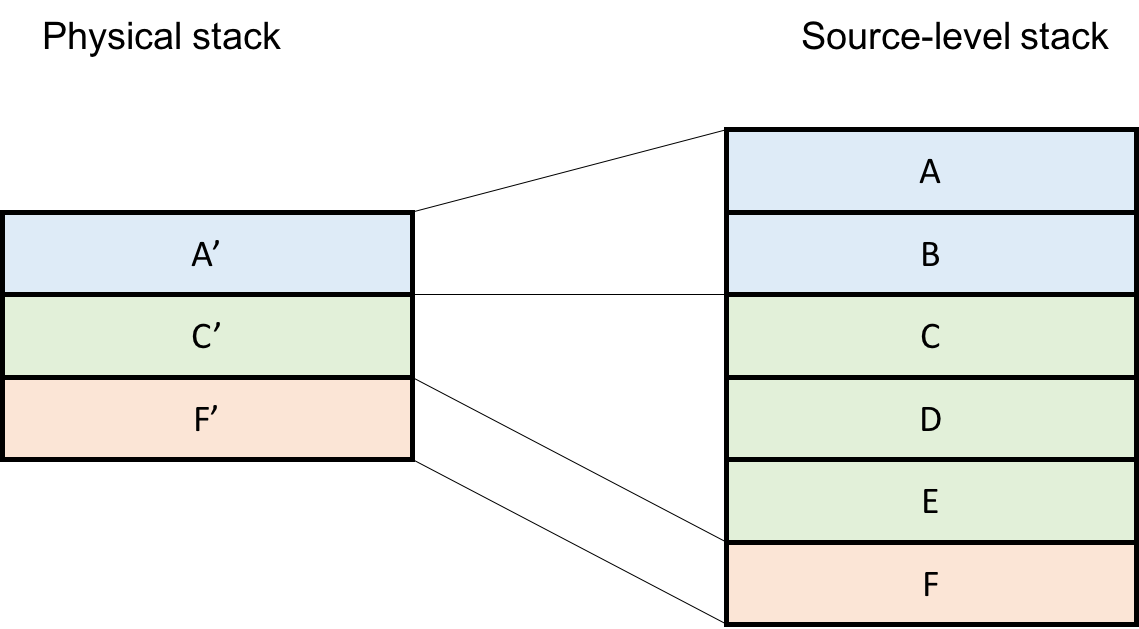
\includegraphics[scale=0.5]{Figures/Figure1}
\decoRule
\caption[physical vs. source-level stacks]{Displaying the stack, figure from \cite{holzle1992debugging}.}
\end{figure}

Single-stepping is another important feature for a debugger. 
It requires to identify and execute the next machine instruction that corresponds to the source operation.
\citean{holzle1992debugging} highlight the impact of code motion and instruction scheduling on the machine instruction layout. 
Such optimizations re-order, merge, intersperse and sometimes delete source-level operations, therefore preventing a straight forward implementation of single-stepping for the debugger.\\

Compiler optimizations prevent dynamic changes from being performed in the debugger.
Holzle(CITE) identifies two separate issues: changing variable values, and modifying procedures (i.e., functions).
To illustrate the first case, Holzle CITE relies on an example where a variable is assigned the sum of two other variables.
The compiler identifies the two variables as being constants and replaces the addition by a direct constant assignment.
A debugger that allows to change variable values at run time would then yield a non correct behaviour if the user modifies one of the two variables. 
This problem does not arise in the case of unoptimized code since the addition is still present. 
For procedures, Holzle CITE describes an example where a function has been inlined by the compiler, but redefined by the user in the debugger.\\

Holzle(CITE) distinguishes two possible states for compiled code: \textit{optimized}, which can be suspended at widely-spaced interrupt points, from which we can reconstruct source-level state, and \textit{unoptimized}, that can be suspended at any source-level operation and is not subjected to any of the above debugging restrictions.\\

In order to deoptimize code on demand, SELF debugger needs to recover the unoptimized state that corresponds to the current optimized one. 
To do so, it relies on a special data structure, called a \textit{scope descriptor}. 
The scope descriptors are generated during compilation for each source-level scope. 
This data structure holds the scope place in the virtual call tree of the physical stack frame and records locations and values of its argument and local variables. 
It further holds locations or values of its subexpressions.
Along with the scope descriptor, the compiler generates a mapping between virtual (i.e, scope descriptor and source position within the scope) and physical program counters (PC).
Figure \ref{Holzle2} is taken from CITE and displays a method suspended at two different points. 
At time t1, the stack trace from the debugger displays frame B, hiding the fact that B was inlined inside of A.
At time t2, D is called by C which is called by A, hence, the debugger displays 3 virtual stack frames instead of only one physical frame.\\

\begin{figure}[h]
\centering
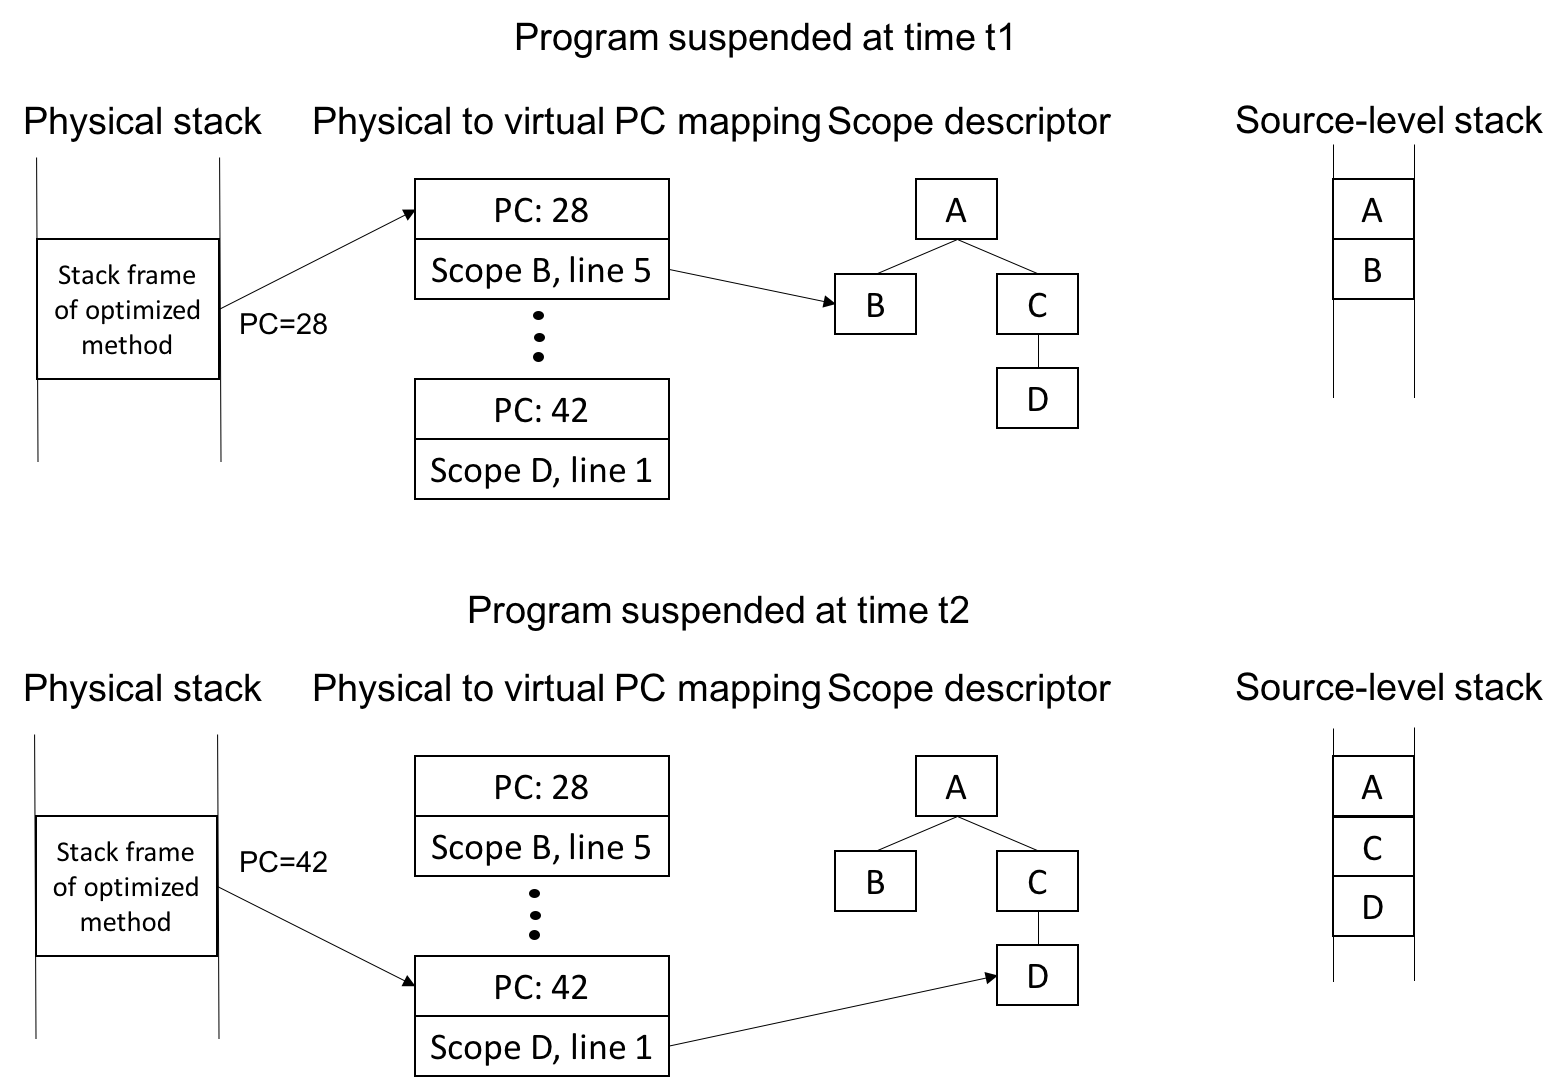
\includegraphics[scale=0.5]{Figures/Figure2}
\decoRule
\caption[Recovering the source-level state]{Recovering the source-level state (from CITE).}
\label{Holzle2}
\end{figure}


The de-optimization process follows 5 steps described in CITE and summed up here:
\begin{enumerate}
    \item Save the physical stack frame and remove it from the run time stack.
    \item Determine the virtual activations in the physical one, the local variables and the virtual PC.
    \item Generate completely unoptimized compiled methods an physical activations for each virtual one.
    \item Find the unique new physical PC for each virtual activation and initialise (e.g., return addresses and frame pointers) the physical activations created in the previous step.
    \item Propagate the values for all elements from the optimized to the unoptimized activations.
\end{enumerate}

Holzle(CITE) also describes \textit{lazy deoptimization}, a technique to deoptimize a stack frame that is not at the current top of the execution stack. 
Lazy deoptimization defers the deoptimization transformation until control is about to return into the frame, hence enabling deoptimization for any frame located on the stack.\\

Deoptimization at any instruction boundary is hard. 
It requires to be able to recover the state at every single point of the program.
Holzle (CITE) relies on a weaker easier restrictions by enabling deoptimization only at certain points called \textit{interrupt points}. 
At an interrupt point, the program state is guaranteed to be consistent. 
The paper (CITE) defines two kinds of interrupt points: method prologues, and backward branches (i.e., end of loop bodies).
Holzle(CITE) therefore estimates the length of the longest code sequence that cannot be interrupted to be a few dozen of instruction, i.e., the average length of a code sequence that does not contain neither a call nor a loop end.
Interrupt points are also inserted at all possible run time errors to allow better debugging of synchronous events such as arithmetic overflow. 
The generated debugging information are needed only at interrupt points, which reduces the space used to support basic debugger operations (as opposed to allowing interrupts at any instruction boundary).\\

Providing a debugger for SELF limits the set of optimizations that the compiler can support, and decreases the performances of the program when the execution is resumed. 
Tail recursion elimination saves stack space by replacing a function call with a goto instruction, while fixing the content of registers.
SELF debugger is unable to reconstruct the stack frames eliminated by this optimization and hence, it is not implemented in the SELF compiler.
More generally, tail call elimination is one important limitation for the SELF debugger.

The debugger slows down the execution when the user decides to resume. 
The execution should proceed at full speed, but some stack frames might have been unoptimized, hence implying that a few frames might run slowly right after resuming execution.\\

\section{OSR \& VMs}
Virtual machines are privileged environments in which On-Stack replacement can be used to its full power.
As seen in \ref{WhyOSRInteresting}, OSR is as useful as the compiler's profiler is efficient.
A virtual machine (VM) has control over the resources allocation, enables to control the code that is generated by the compiler, maintains important run time data, and state information about the program being executed.\\

This section presents several examples of VMs that support On-Stack replacement. 
The section is divided into two parts: we first presents several solutions that provide OSR for various virtual machines, then we briefly introduce LLVM, a VM presenting an interesting framework in which we believe On-Stack replacement mechanism should fit.\\ 

\subsection{HotSpot}\label{HotSpot}

The Java HotSpot Performance Engine(CITE web) is a Java virtual machine developed and maintained by Oracle.
The Java HotSpot VM provides features such as a class loader, a bytecode interpreter, Client and Server virtual machines, several garbage collectors, just-in-time compilation and adaptive optimizations.\\

The Java HotSpot Engine supports on-stack replacement in order to provide efficient deoptimization\cite{paleczny2001java}.
When a class loading invalidates an optimization decision, such as a call inlining, the methods relying on this decision need to be deoptimized.
Threads that are executing in a method that needs to be deoptimized are stopped as soon as they reach a safepoint.
The JVM state is recorded as an input of safepoints and procedure calls.
This implies, as a side effect, that the entire JVM state is marked as "live" at a safepoint, hence extending the live range of some values.
The Java HotSpot Engine then extracts the native frame corresponding to this execution trace, and converts it into a byte code interpreter frame.
The execution of the method then continues in the interpreter.
UNCOMMON TRAPS\\

\subsection{Jikes RVM}

The Jikes Research Virtual Machine (RVM)(REF) is an open source, self hosted, i.e., it is entirely implemented in Java, virtual machine for Java programs.
%TODO compile only from Qian.
It provides advanced state-of-the-art features such as dynamic compilation, adaptive optimizations, garbage collection, thread scheduling, and synchronization (CITE).\\

Jikes RVM is an extensible framework in which different On-Stack replacement techniques have been implemented.
%The first
\citean{fink2003design} implemented OSR support in JikesRVM. 
Their implementation relies on JVM scope descriptor, associated to method activation frames.
A scope descriptor contains the thread running the activation, the bytecode index that corresponds to the program counter, values of all local and stack locations, and a reference to the activation's stack frame.
The OSR transition is divided into three steps: 
\begin{enumerate}
    \item Extract the compiler-independent state from a suspended thread. 
    \item Generate the new code for the suspended activation.
    \item Transfer the execution in the suspended thread to a new compiled code.
\end{enumerate}
\citean{fink2003design} generates the target function by compiling a specialized version of the method for each activation that is replaced, as well as a new version for future invocations.
In other words, instead of allowing multiple entry points per function \cite{lameed2013modular, paleczny2001java}, this JikesRVM OSR implementation generates a specialized version of the target function that has only one entry point, corresponding to the instruction from which the OSR transition was triggered.
Each such method contains a special \textit{prologue}, responsible for saving values into locals and loading values on the stack.
OSR transitions can be taken at special points, called \textit{OSR points}, introduced by the optimizing compiler and that correspond to points where the running activation may be interrupted.
The implementation makes a distinction between unconditional and conditional OSR points.
An OSR point is implemented as a call that takes all live variables as arguments. 
This constraints some optimizations such as dead code elimination, load elimination, store elimination and code motion by extending the liveness scope of some variables.
An OSR point transfers control to an exit block, i.e., it can be viewed as a non-return call.\\

\citean{soman2006efficient} proposed a general-purpose OSR mechanism, for JikesRVM, that presents less restrictions for compiler optimizations than the previous approach, while decoupling the OSR implementation from the optimization process.
They extend the previous OSR implementation\cite{fink2003design} to enable OSR transition at, and accross points at which the execution can be suspended.
In order to do so, they rely on a special data structure called a \textit{variable map}(VARMAP).
A VARMAP is associated with each method, and consists in a list of thread-switching points and their live variables.
When the compiler performs optimizations, the VARMAP is updated accordingly.
Once the compilation completes, the VARMAP is encoded into a compressed map that contains an entry for each OSR point present in the method. EXPAND ON HOW OSR IS PERFORMED.
\citean{soman2006efficient} also propose an alternative lazy triggering of on-stack replacement.
Lazy triggering consists in taking an OSR transition due to events in the environment, i.e., events triggered by the runtime. 
Whenever the runtime deems an assumption invalide, it invokes a helper function called \textit{OSR helper} that either patches the code of the executing methods to call the OSR process, or it modifies return addresses of the callees of the method to be replaced to point to the OSR helper.
When a callee returns, the OSR helper creates a new stack frame with the state extracted from the specialized method's stack and saves all of the specialized method registers into its stack frame. 
The return address of the OSR helper points to the current instruction in the specialized code, which is then used during OSR to identify the location to resume the execution in the new version of the method.
Lazy triggering improves the code efficiency by avoiding the extra cost of guards evaluations.\\

EXPERIMENTAL RESULTS.

\subsection{WebKit VM}\label{webkit}

WebKit is an open source web browser engine used to improve JavaScript performances.
It exhibits a Four-Tier VM architecture. 
The WebKit run-time compilation flow is described by Figure \ref{FTL}.\\
\begin{figure}[h]
\centering
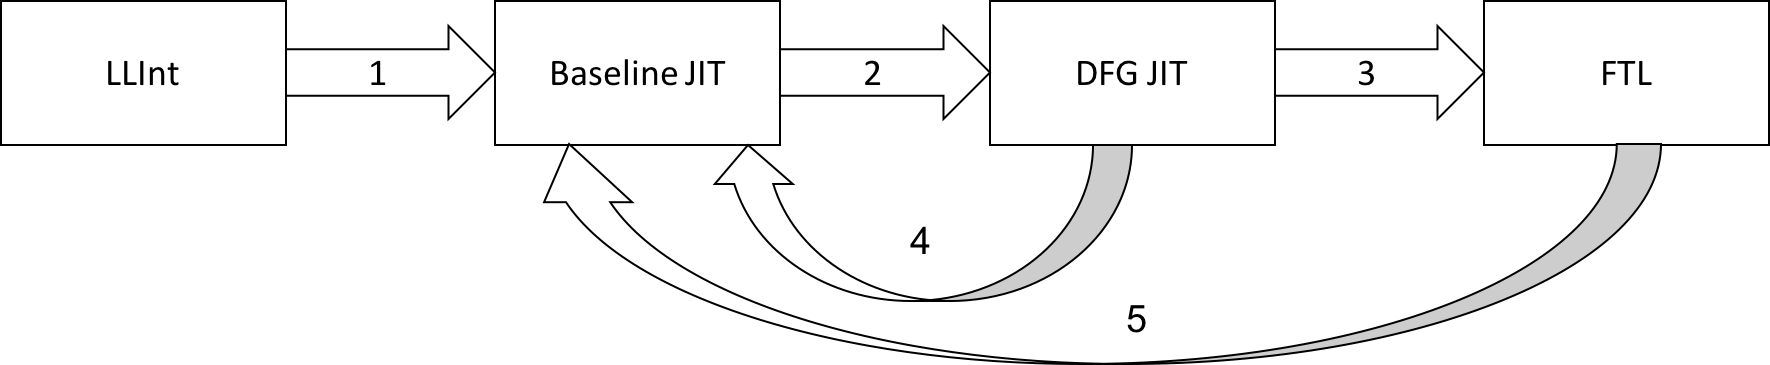
\includegraphics[scale=0.5]{Figures/FTL}
\decoRule
\caption[The WebKit FTL]{The WebKit Four-tier optimization flow.}
\label{FTL}
\end{figure}
 
Forward arrows represent \textit{OSR entries}, i.e., a transformation that yields a more optimized version of the code at run-time.
Backward arrows correspond to \textit{OSR exits}, i.e., a transformation that yields a less optimized version of the code at run-time.
The low level interpreter (LLInt) is used for low latency start up.
The baseline JIT generates WebKit bytecode with no optimization enabled.
The transition from the first tier to the second one happens when a statement is executed more than a hundred times or a function is called more than six times.
The data flow graph (DFG) JIT is triggered when a statement executes more than a thousand times or a function is called more than sixty-six times.
The FTL tier relies on LLVM machine code optimizations to generate a fast version of portions of the code.
In order to hide the costs of the translation to LLVM IR and its compilation time, the FTL is triggered only for long running portions of the code that are currently executing.
There are two kinds of transitions in WebKit: the ones contained entirely inside the WebKit framework (i.e., transitions 1,2 \& 4 in Figure \ref{FTL}), and the ones that involve LLVM (i.e., 3 \& 5 in Figure \ref{FTL}).\\

Transitions to and from LLVM are hard. 
There is no control over the stack layout or the optimized code produced by LLVM.
In the case of transition 3, a different LLVM version is generated for each entry point that the framework desires to have inside this function.
In WebKit, such entry points are located at loop headers. 
This choice makes sense with regard to the condition to enter the FTL, i.e., transition 3 is taken for long running portions of code that could be improved thanks to LLVM low level optimizations.
WebKit has to generate a different version for each entry points for two main reasons: LLVM allows only single entry points to functions (going around this limitation would require to modify LLVM IR and implementation), and instrumenting a function with several entry points would impact on the quality and performance of the generated native code by extending the code's length and restricting code motion.\\

Performing transition 3 requires to get the current state of execution and identify the entry point corresponding to the current instruction being executed.
The DFG dumps its state into a scratch buffer.
An LLVM function with the correct entry point is then generated, and instrumented such that its first block loads the content of the scratch buffer and correctly reconstructs the state.
The mapping between the DFG IR nodes and the LLVM IR values is straight forward since both IR's are in SSA.
A special data structure, called a Stackmap, enables to keep the mapping between LLVM values and registers/spill-slots.\\

Transition 5 is harder as it requires to extract the execution state from LLVM.
WebKit has two different mechanisms to enables OSR exits: the exit thunk and the invalidation points.
In the first case, WebKit introduces exit branches at OSR exit points.
The branch is guarded by an OSR exit condition and is a no-return tail call to a special function that takes all the live non-constant and not accounted for bytecode values.
The second mechanism enables to remove the guard.
Since we assume that the portion of code that is instrumented is executed a lot of times, the cost of testing the condition can have a great impact on the overall execution time.
This mechanism relies on special LLVM intrinsics, namely patchpoints and stackmap shadow bytes.
A patchpoint enables to reserve some extra space in the code, filled with nop sleds. 
When the WebKit framework detects that an exit should be taken, it overwrites the nop sleds with the correct function call to perform the OSR exit.
This breaks the optimized version of the code which cannot be re-used later on and must be collected.
The stackmap shadow bytes improves on this technique by allowing to directly overwrite the code, without having any nop sled generated before hand.

WebKit is a project that heavily, and successfully relies on OSR to improve performances.
The web browser engine is used in Apple Web browser Safari and enables a net improvement of performances why proving to be reliable(CITE?).
Although successful, it does not provide a general and reusable framework for OSR in LLVM that other projects could benefit from.\\

\section{OSR \& LLVM}\label{OSR&VM}
\subsection{What is LLVM?}
%TODO cite the llvm paper?
LLVM is a compiler infrastructure providing a set of reusable libraries.
LLVM provides the middle layers of a compiler system and a large set of optimizations for compile-time, link-time, run-time, and idle-time for arbitrary programming languages.
These optimizations are performed on an intermediate representation (IR) of the code and yield an optimized IR.
The LLVM framework also provides tools to convert and link code into machine dependent assembly code for a specific target platform.
LLVM supports several instruction sets including ARM, MIPS, AMD TeraScale, and x86/x86-64(CITE?).\\

The LLVM intermediary representation is a language-independent set of instructions that also provides a type system.
The LLVM IR is in static single assignment form (SSA), which requires every variable to be defined before it is used and assigned exactly once. 
SSA enables or improves several compiler optimizations among which constant propagation, value range propagation, sparse conditional constant propagation, dead code elimination, global value numbering, partial redundancy elimination, strength reduction and register allocation.
The SSA requirement for variables to be assigned only once requires a special mechanism, called a $\phi$-node, when a value depends on which control flow branch was executed before reaching the current variable definition.
Figure \ref{SSA example} provides an example where we have to choose between two possible values for a variable after the merging of two control flow branches.

\begin{figure}[h]
\centering
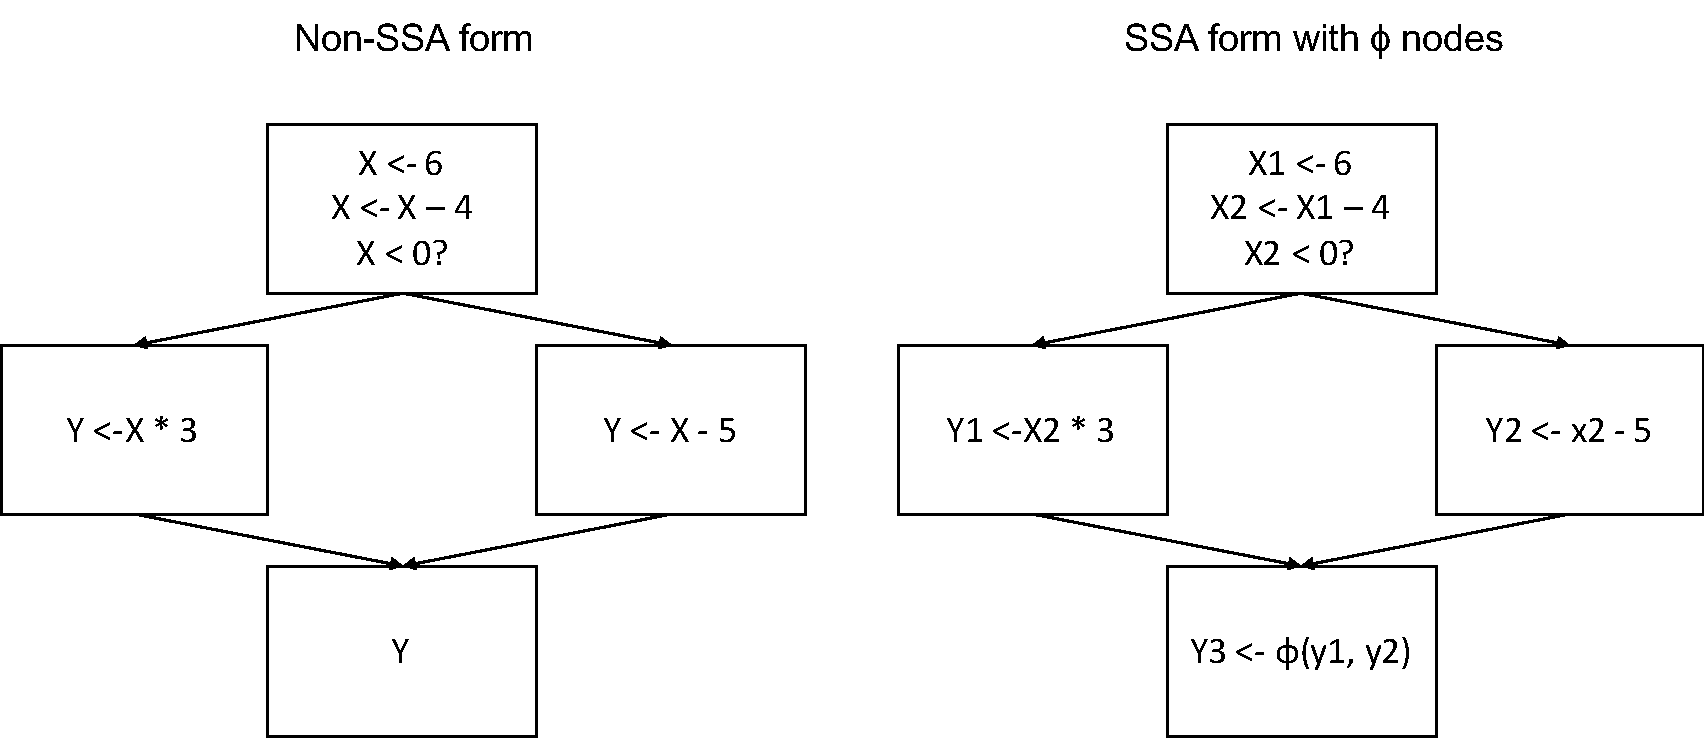
\includegraphics[scale=0.5]{Figures/SSAForm}
\decoRule
\caption[SSA example]{Example of $\phi$-node in SSA form.}
\label{SSA example}
\end{figure}

%TODO exhaustive basic types?
The LLVM IR type system provides basic types (e.g., integers, floats), and five derived types: pointers, arrays, vectors, structures, and functions.
Any type construct can then be represented as a combination of these types.\\

%TODO reformulate/restructure this §
The LLVM framework is a versatile tool that enables to implement many programming languages paradigms.
LLVM compilers exist for several mainstream/popular languages such as Java, Python, Objective-C, and Ruby have an LLVM compiler.
Other languages, like Haskell, Scala, Swift, Rust, Ada, and Fortran also have an LLVM compiler implementation.
LLVM basic types enable to support object-oriented languages, such as Java and Python, dynamically typed languages like R or statically typed like Scala.
LLVM also enables to model functional languages such as Haskell, as well as imperative ones. 
Furthermore, it supports reflection and, thanks to dynamic linking, modular languages (e.g., Haskell).
The tools provided enable static compilation as well as dynamic compilation techniques such as Just-In-Time compilation (JIT).\\

\subsection{Why do we want OSR in LLVM?}

On-Stack replacement high-level mechanism is language-independent.
Therefore, implementing OSR as a clean modular addition to LLVM would enable developers to leverage this feature in many programming languages, without requiring them to write a new compiler from scratch.
Furthermore, as explained in \ref{WhyOSRInteresting}, OSR is a useful tool for dynamic and adaptative optimizations.
LLVM already provides implementations for many compiler optimizations(CITE) and tools to allow dynamic recompilation of code.
Developers can therefore focus on language specific challenges, such as efficient profilers and new speculative systems, rather than on the optimizations and OSR implementations.

Implementing OSR for LLVM not only serves several languages, but also allows to provide a solution for several target platforms.
As explained previously, LLVM supports several instructions sets corresponding to different architectures.
By implementing OSR in LLVM, we get portability among these platforms for free.\\

\subsection{OSR as an LLVM library: the MCJIT OSR implementation}\label{McJIT}
The MCJIT OSR support(CITE) is an attempt at providing an OSR library compatible with the standard LLVM implementation.
Lameed \& Hendren claim to have come up with a clean modular, and re-usable technique completely defined at the LLVM IR level and compatible with the standard LLVM distribution.
There implementation answers to five challenges, listed in the paper CITE and that we reproduce here:\\ 

\begin{enumerate}
    \item Identifying correct interrupt points and using the current LLVM IR to represent them.
    \item Using the LLVM tools to correctly transform the IR while preserving a correct control flow graph. 
    \item Making a new version of a function available at the same address as the old one.
    \item Providing a clean API for the OSR library, that is compatible with LLVM's inlining capabilities.
    \item Integrating OSR without modifying the LLVM installation.
\end{enumerate}

The paper (CITE) claims to support optimization and re-optimization, as well as de-optimization by going back to the previous version of the function.
Figure \ref{OSR classification} shows that this feature only allows single-steps to be taken, i.e., the OSR library implemented in CITE does not seem to allow to skip intermediary versions.\\

\begin{figure}[h]
\centering
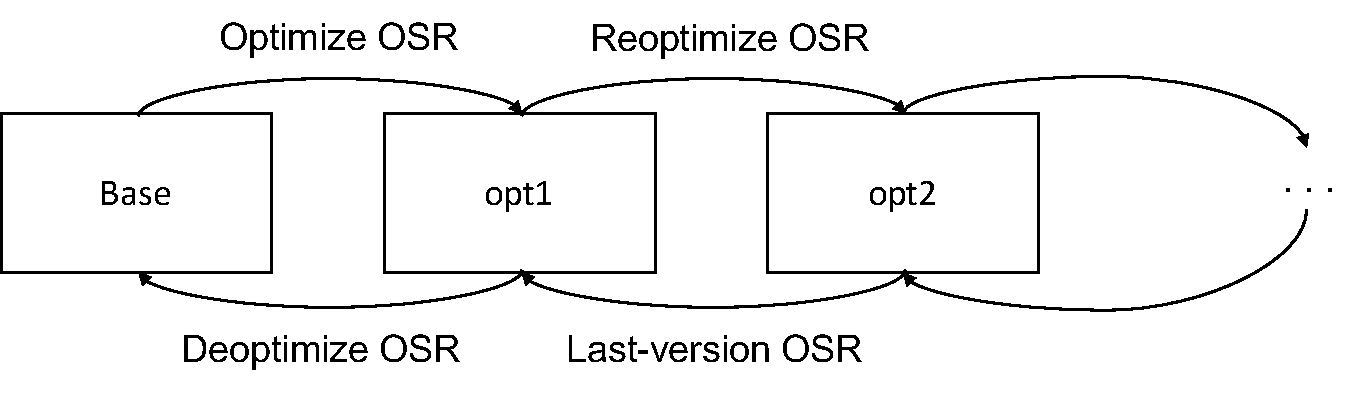
\includegraphics[scale=0.5]{Figures/OSRClassification}
\decoRule
\caption[OSR classification]{OSR classification from CITE}
\label{OSR classification}
\end{figure}

The MCJit library that provides OSR functionalities fit into the regular JIT infrastructure provided by LLVM as described in Figure \ref{MCJitArchitecture} taken from CITE. 
\begin{figure}[h]
\centering
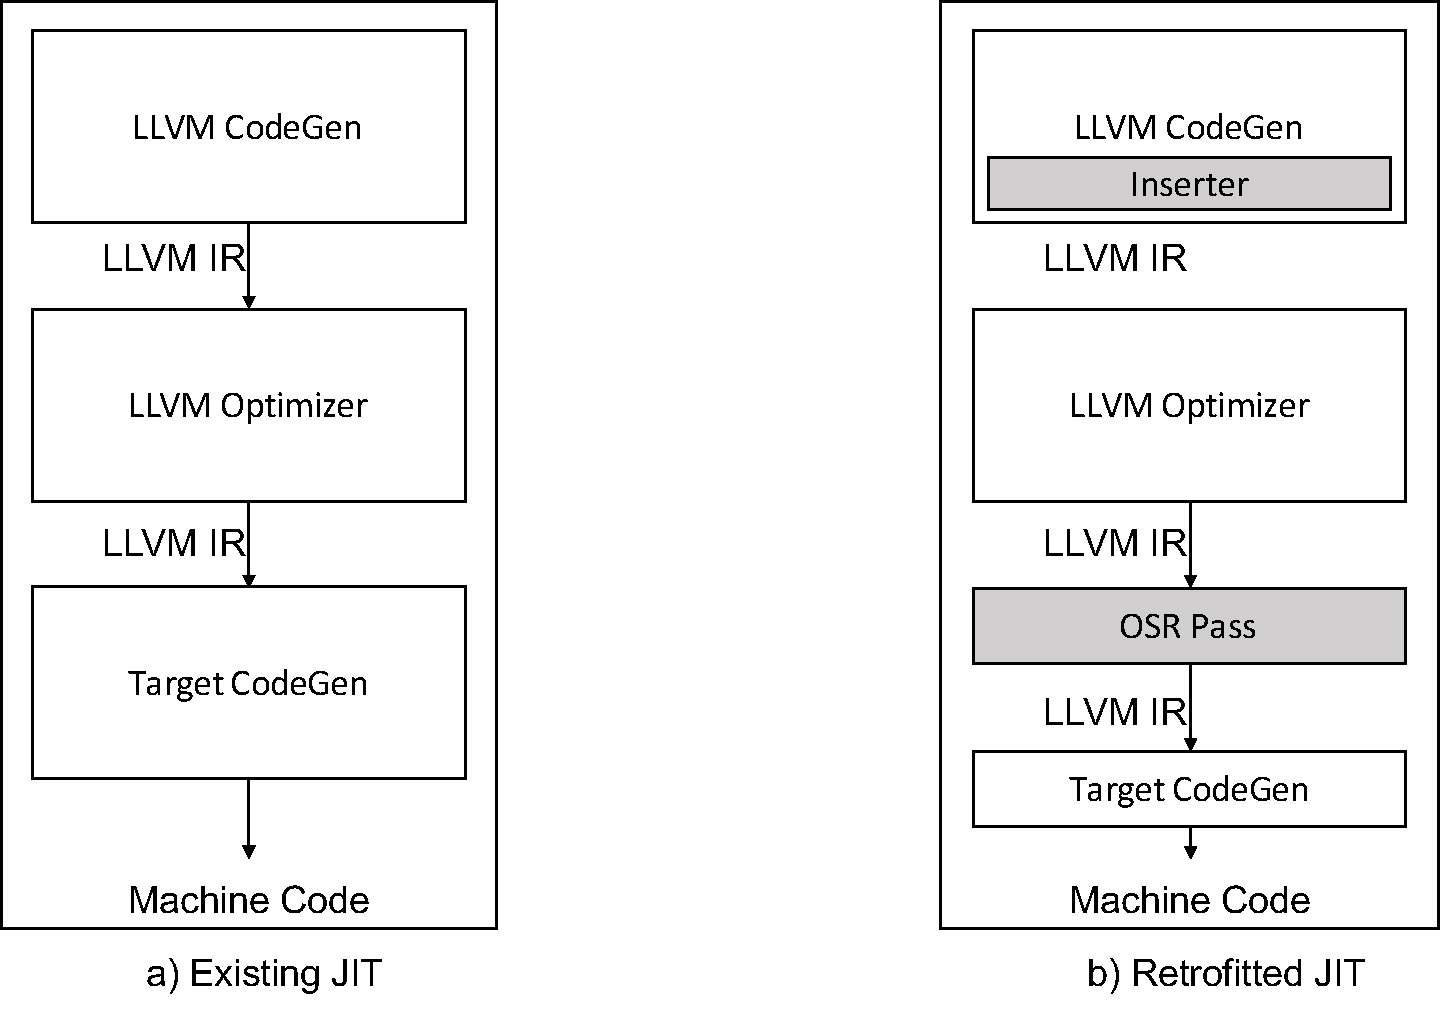
\includegraphics[scale=0.5]{Figures/MCJitArchitecture}
\decoRule
\caption[Retrofitting an existing JIT with OSR support]{Retrofitting an existing JIT with OSR support from CITE}
\label{MCJitArchitecture}
\end{figure}
The left figure is a normal JIT in LLVM. 
The LLVM CodeGen is the front-end of the compiler infrastructure that generates the LLVM IR.
The LLVM Optimizer contains a collection of transformations and optimizations that run on LLVM IR. 
The Target CodeGen outputs the machine code corresponding to the LLVM IR input. 
The MCJit OSR API instruments the LLVM CodeGen to insert OSR points where the OSR transition can be triggered. 
A point is a call to the genOSRSignal function, which takes as arguments a pointer to a code transformer responsible for generating the new version of the function.
The code transformer takes as arguments a pointer to the function that needs to be transformed, and a special OSR label to identify which OSR points triggered the call, if the function contains several ones.
The OSR pass is responsible for instrumenting OSR points with the correct OSR machinery.
The instrumentation saves the live values and creates a descriptor that contains four elements: 
%TODO explain the control version better
\begin{enumerate}
    \item A pointer to the current version of the function. 
    \item A pointer to the control version of the function, i.e., a copy of the old version of the function.
    \item A variable mapping between the original version and the control version.
    \item The set of live variables at the OSR points. 
\end{enumerate}\\

\begin{figure}[h]
\centering
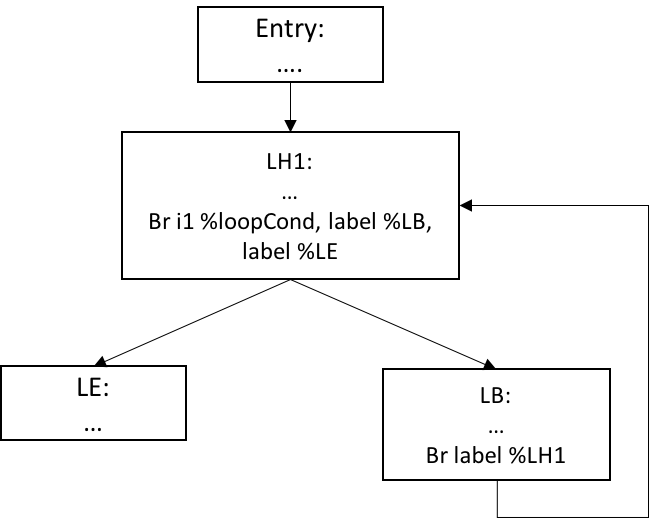
\includegraphics[scale=0.5]{Figures/BaseCFG}
\decoRule
\caption[A CFG of a loop with no OSR point]{A CFG of a loop with no OSR point from CITE.}
\label{BaseCFG}
\end{figure}

\begin{figure}[h]
\centering
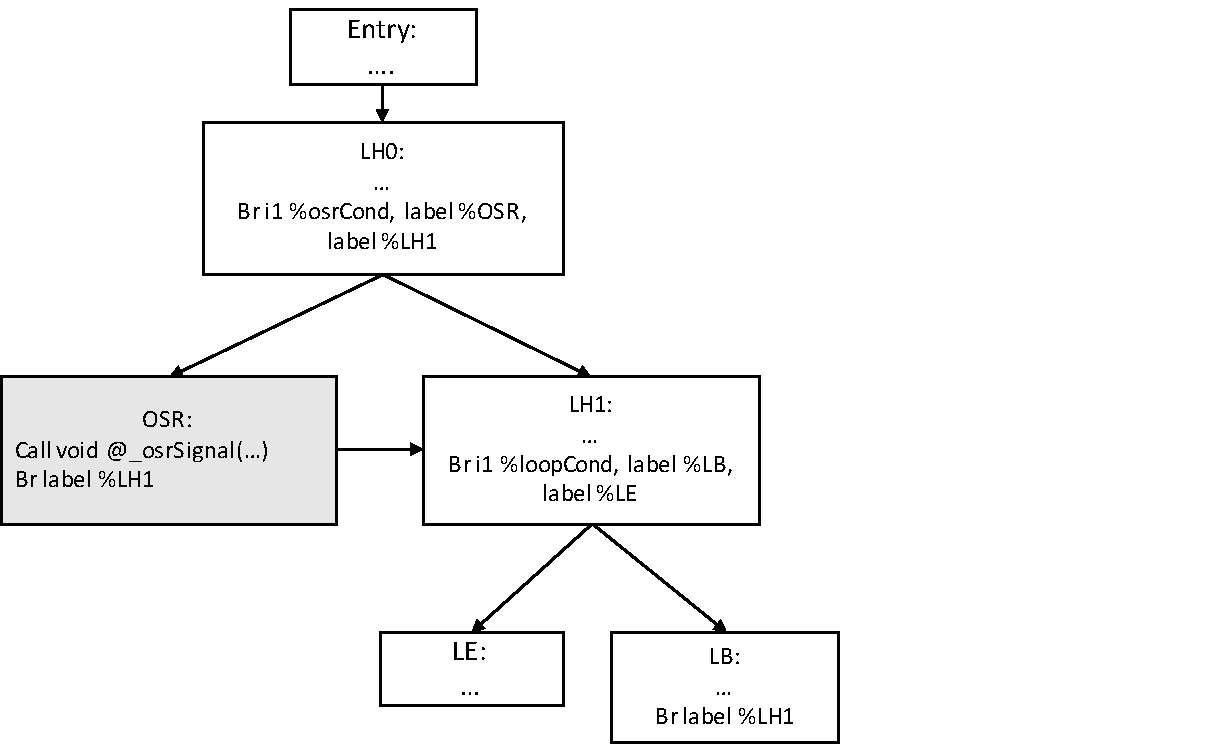
\includegraphics[scale=0.5]{Figures/InsertCFG}
\decoRule
\caption[The CFG of the loop in Figure \ref{BaseCFG}, after inserting an OSR point]{The CFG of the loop in Figure \ref{BaseCFG}, after inserting an OSR point from CITE.}
\label{InsertCFG}
\end{figure}

\begin{figure}[h]
\centering
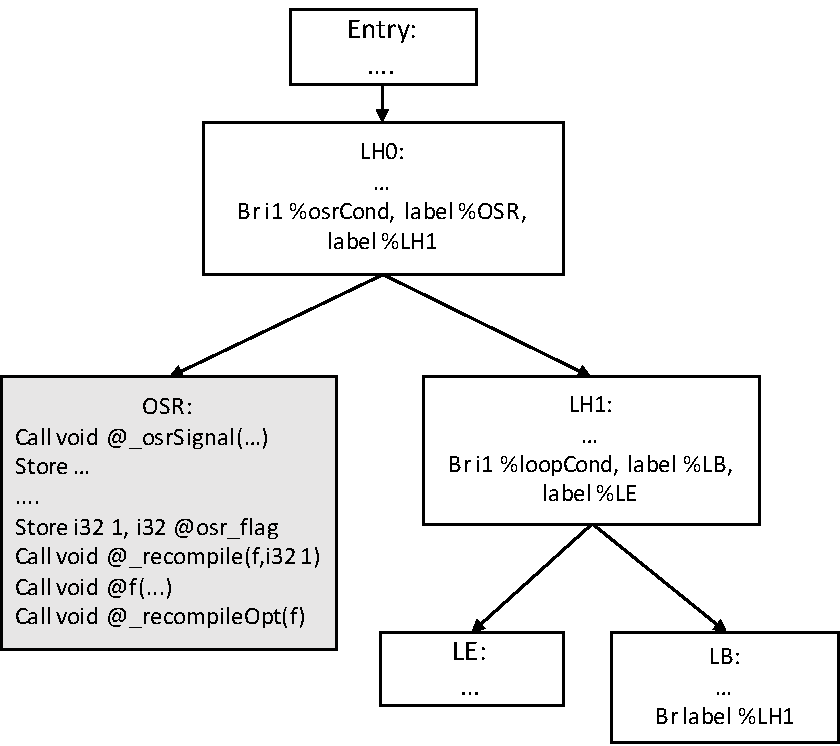
\includegraphics[scale=0.5]{Figures/OSRPassCFG}
\decoRule
\caption[The transformed CFG of the loop in Figure \ref{InsertCFG} after the OSR Pass]{The transformed CFG of the loop in Figure \ref{InsertCFG} after the OSR Pass from CITE.}
\label{OSRPassCFG}
\end{figure}\\

Figures \ref{BaseCFG}, \ref{InsertCFG}, and \ref{OSRPassCFG} give an example of OSR instrumentation at a loop header.
LH1 is the loop header. 
LB is the body of the loop and LE the loop exit. 
Figure \ref{BaseCFG} control flow graph (CFG) is the original CFG. 
Figure \ref{InsertCFG} is the resulting CFG after the Inserter is executed.
Figure \ref{OSRPassCFG}'s CFG corresponds to the result of the OSR pass.
The \textit{recompile} call in the OSR block recompiles \textit{f} using the correct code transformer.
Then \textit{f} calls itself, executing the new version of the function.
This works since the new version lives at the same address as the previous one and is instrumented to jump to the correct instruction, i.e., the one corresponding to the current point at which OSR was triggered.
Figure \ref{FCFG} represents the CFG of \textit{f} before the OSR instrumentation.
Figure \ref{InstFCFG} shows the instrumentation of \textit{f} that enables to jump to the correct instruction in the middle of the function. 
A prolog entry block is inserted at the function header.
This block checks the \textit{OSR flag} to know if an OSR transition is being performed.
If that is the case, it branches to the prolog block that restores the state before resuming the execution at the correct instruction.\\

\begin{figure}[h]
\centering
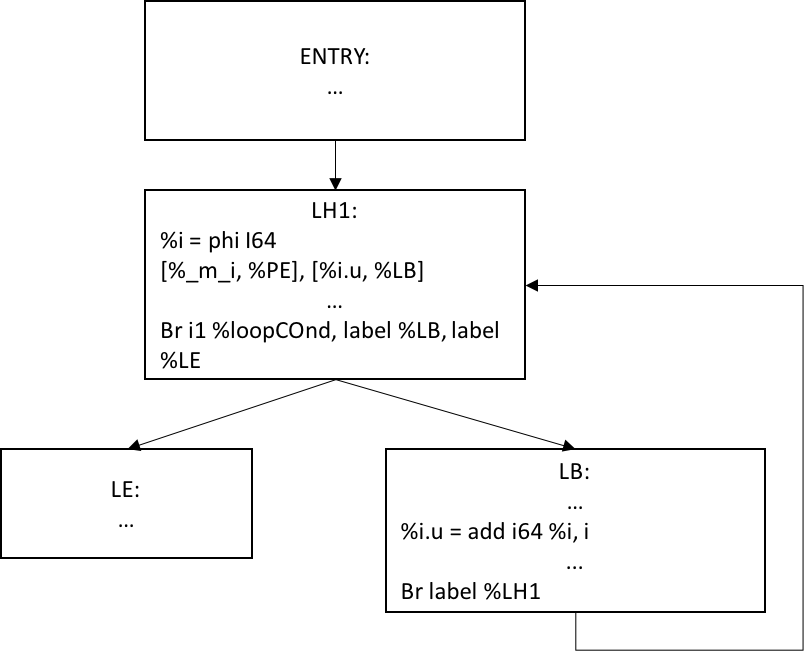
\includegraphics[scale=0.5]{Figures/FCFG}
\decoRule
\caption[A CFG of a running function before inserting the blocks for state recovery]{A CFG of a running function before inserting the blocks for state recovery, from CITE.}
\label{FCFG}
\end{figure}

\begin{figure}[h]
\centering
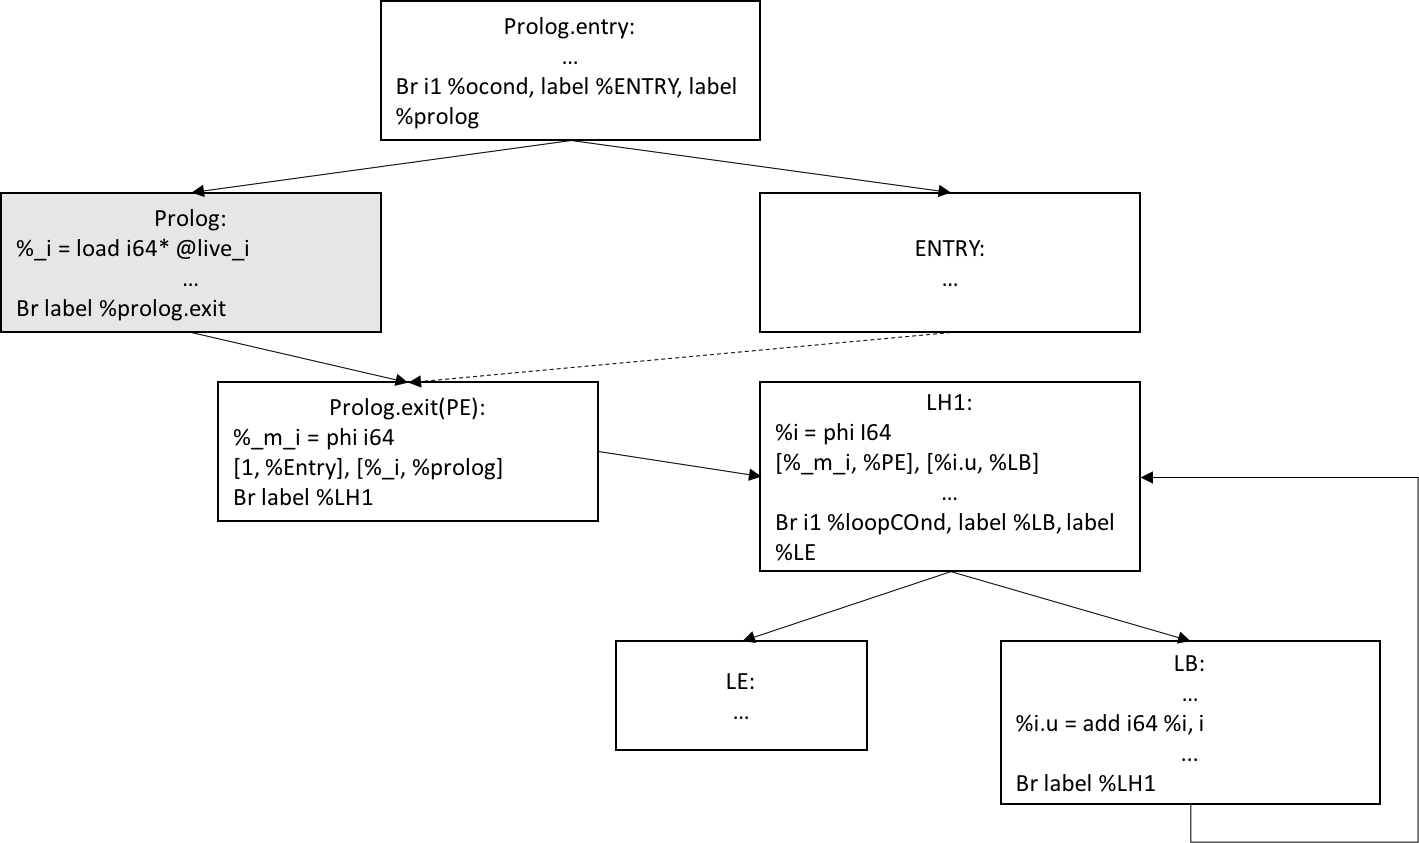
\includegraphics[scale=0.5]{Figures/FOptCFG}
\decoRule
\caption[The CFG of the loop represented in Figure \ref{FCFG} after inserting the state recovery blocks, form CITE.]{The CFG of the loop represented in Figure \ref{FCFG} after inserting the state recovery blocks, form CITE.}
\label{InstFCFG}
\end{figure}\\

%TODO critic of the paper.
The OSR implementation proposed in CITE presents interesting features.
The implementation is done entirely at the LLVM IR, hence making it language-independent.
Furthermore, since the transformation function is provided by the user, any kind of language specific transformation can be used during the OSR.
As a result, MCJit OSR support is an interesting modular OSR library.

On the other hand, this library does not allow to have several versions of the same function, live at the same time.
This restriction can impede the overall performance of the program by extending the scope in which an assumption on which we base the transformation must hold.
For example, a portion of the code, call it \textit{A}, can trigger an OSR, while portion \textit{B} is such that the assumption on which the optimization is based does not hold.
The choice that the user has is to either optimize for A, and deoptimize for B, or to prevent A from optimizing by enlarging the scope in which the assumption is supposed to hold.
None of these solutions is good if \textit{A} and \textit{B} are executed many times, one after the other.
We will either lose a lot of execution time performing OSR, or keep executing \textit{A} without optimization.

In the paper, the deoptimization process is not described. 
It is implied that it relies on the same set of tools provided by the framework as the optimization process, but no example is provided.
As explained in \ref{WhyOSRInteresting}, deoptimization is the most interesting feature of OSR, as it is required to preserve correctness.
Being able to identify where a function should exit is a hard task.
The MCJit library does not provide tools to ease this process and leaves the responsibility to the developer to instrument his functions correctly in order to exit to the correct landing pad.

To the best of our knowledge, MCJit OSR library is not currently used in production or any important project.
As mentioned earlier, WebKit is efficiently integrated in Apple Safari's web browser, which provides useful feedback on its performances.
The lack of usage of MCJit OSR library prevents us from collecting performance results and assess its efficiency.
Furthermore, the experimental evaluation in CITE relies on an example that seems artificial for our use of OSR. 
The case study presents a dynamic inliner that decides to inline a function call if the function is less than 20 basic blocks long, or if it is less than 50 basic blocks long and has an interpreter environment associated with its body. 
This requirement for inlining is one that can be checked statically and, hence, seems a little artificial.\\

\section{A classification summary}
%TODO some kind of sum up and comparison, related to what we had in chapter 2.

% Chapter 4

\chapter{OSR in RJIT} % Main chapter title

\label{Chapter4New} % For referencing the chapter elsewhere

%----------------------------------------------------------------------------------------

% Define some commands to keep the formatting separated from the content 
\newcommand{\keyword}[1]{\textbf{#1}}
\newcommand{\tabhead}[1]{\textbf{#1}}
\newcommand{\code}[1]{\texttt{#1}}
\newcommand{\file}[1]{\texttt{\bfseries#1}}
\newcommand{\option}[1]{\texttt{\itshape#1}}

%----------------------------------------------------------------------------------------
\section{Overview}
\subsection{The RJIT compiler}
\subsubsection{General}
CITE GNUR\\
%General information
The RJIT project is an LLVM based JIT Compiler for the R programming language.
It relies on GNUR, an interpreter for R. 
The RJIT compiler takes as input a symbolic expression (SEXP), i.e., a special C structure generated by GNUR while parsing R programs.
A SEXP represents R constructs and contains the AST representation of an R element.
A SEXP has a type, and can be seen as a lisp-like cons cells, composed of two pointers, CAR and CDR.
A SEXP has many other elements, that we do not detail here.
Depending on its type, each SEXP element corresponds to a specific attribute (see examples for closures and functions below). 
The GNUR interpreter has been instrumented to call the JIT compiler before evaluating a non-compiled SEXP. 
The RJIT compiler generates native code, using the LLVM framework, that corresponds to the R function's AST it received as argument.
The native code is then wrapped into the appropriated SEXP constructs, and returned to the GNUR interpreter.
Afterwards, the GNUR interpreter executes the native code.\\ 
%Compilation flow

\subsubsection{The RJIT compilation flow}
%intrinsics 
%Constant pools for local variables
%All functions have the same signature !
%promises !!!
RJIT walks the SEXP ast and generates the corresponding LLVM IR.
Since R is a dynamic language, most R constructs need to be simulated by LLVM calls to special functions, called R intrinsics.
CONTINUE THIS PART.\\

IC CALLEE IS WRAPPER, DESCRIBE BETTER\\
%ic stubs.
R resolves callee of function calls at runtime, when the call is executed.
In order to simulate this behavior, the RJIT compiler needs to rely on a special instrumentation to compile calls to functions that are not yet resolved.
To that end, the JIT compiler replaces function calls with inlined cached stubs (i.e., ic stubs).
An ic stub takes as parameters the function call's arguments, a pointer to the callee extracted from the environment, and a pointer to the caller.
The ic stub, when executed, compiles a special function that caches the resolved callee, call it the ic callee.
This function is instrumented to check, during future calls, that the resolved function for the callee is the same as the one it saw during its own compilation, and performs the call.
Once the ic callee is compiled, the ic stub replaces itself in the caller with a direct call to the ic callee.
In order to do so, the ic stub relies on LLVM intrinsics called Stackmap REF, patchpoints REF, and on the caller's pointer it received as argument.\\

\subsubsection{The function's SEXP}
In GNUR and RJIT, a function is represented by a special SEXP. 
This SEXP has a NATIVESXP type when the function is compiled by the RJIT compiler, and a LANGSXP, i.e., a language construct, when it is not.
In the case of a compiled function, the CDR element contains a pointer to the native code of the function.
In the case of a non-compiled function, the CDR contains the AST of the function.
The CAR element, in both cases, contains the constant pool associated to the function, i.e., the list of symbols defined inside the function.
For a compiled function, the TAG element of the SEXP contains the LLVM IR of the function.\\

When the GNUR interpreter evaluates a function SEXP, it checks the SEXP type. 
If the function is compiled, it performs the call to the native code. 
If not, it calls the RJIT compiler, and calls the resulting native code.\\

\subsubsection{The closure's SEXP}
In R, a closure contains a function and the environment associated to it.
A closure SEXP has type CLOSXP.
The CAR of a SEXP closure is a function SEXP.
The CDR of a SEXP closure is an environment SEXP, of type ENVSXP.
A closure also contains the formals, i.e., the arguments symbols of the function.
The getFunction intrinsic, that enables to resolve a function, returns a closure.
The environment is made of cons cells, and is essential to the execution of a function.
Local variables and function argument values are set inside the environment.\\

\subsection{Justification \& Goals}
REWRITE - REFORMULATE.\\
%Goal of the thesis 
    %on stack replacement general mechanism, reusable, at llvm level
    %Why? improve performance and allow greater flexibility in RJIT
        %R is slow, 
        %R is a dynamic language lots of difficulties for implement opt
        %Hence OSR. 
%Reuse an existing library to focus on deoptimization
    %Our goal is to aggressively optimize while preserving correctness
    %Project still young, don't know exactly what we need, don't have feedback on the code
    %Hence better to reuse lib that we can modifiy -> OSR Kit 
%Restate goals 
    %Try to specialise the OSR Kit for the deopt and overcome the limitations. 
    %Will test it with an inlining. 
            

The goal of this Master Thesis project is to provide a flexible OSR deoptimization framework in LLVM, and use it to improve performances in RJIT, our LLVM JIT compiler for R.
R is a programming language and software environment for the statistical computing and graphics, developed by the R Foundation for Statistical Computing\cite{RURL}.
Due to SAY WHYYYYYYYYYYYYYYYYYYYYYYYYYY OOOOOHHHHH GOOOOOOODDDDDD WHHHYYYYYYYYYY, R exhibits very poor performances CITE SOMETHING.
The RJIT project strives to improve these performances by providing a LLVM based JIT compiler for R. SAY MORE.
The RJIT compiler is still pretty young, only a few months old.
As a result, we lack FEEDBACK; DONT KNOW EXACTLY HOW TO IMPROVE PERF AND NEED TO EXPERIMENT.
Therefore, we are looking for a flexible and extensible OSR mechanism that enables us to prototype and experiment various solutions, without trapping ourselves into a single model.\\

The OSR Kit library\cite{OSRKit} is a flexible implementation of on-stack replacement instrumentation in LLVM.
The source-code for the library is available on Github\cite{OSRKitGit}, and the library can be used in any LLVM project by simply copy-pasting the OSR Kit files inside of it.
The simple integration, the availability of the source code, and the flexibility of the framework make it a perfect base implementation upon which we can implement our support for OSR deoptimization mechanisms in RJIT.\\

OSR Kit library enables to work at the LLVM IR level.
LLVM IR is a stable representation that combines the advantages of both the high-level representation, i.e., it still contains some semantic constructions particular to the language being compiled, and the advantages of a lower level representation, closer to the execution engine.
In the case of this master thesis project, i.e., providing OSR mechanisms in the RJIT project, the LLVM IR is the exact middle layer representation that we need. 
At the LLVM IR level, the R semantics are still visible and it therefore allows us to efficiently implement our optimizations.\\

%TODO MORE ABOUT THE FOCUS ON DEOPT. 
MOVE UP\\

This master project thesis focuses on the design and implementation of a prototype for OSR deoptimization support in RJIT.
Starting a new OSR transition implementation from scratch requires time.
Using a flexible and modifiable OSR transition library therefore seemed like the goto option.
We do not waste time reimplementing something that already exists, and can therefore put all our efforts into implementing an interesting OSR deoptimization case, testing it, and extending the OSR Kit library with mechanisms that are specific to our needs (Sections \ref{osrForUs} and \ref{extendingOSR}).\\

\subsection{OSR Kit limitations}\label{osrkitlimitations}

%While very flexible, comes short on several points
    %Open OSR, not really fitting our case.
    %Continuation style is fine for optimization, but pretty bad for deopt.
        %no replacement when exits... 
        %many clones ... 
        %As we'll see later, cloning is not sufficient ...
While very flexible, the OSR Kit\cite{OSRKit} library presents several disadvantages and exhibits costly behaviors that do not perfectly fit the deoptimization process.
This section lists the challenges encountered while trying to implement OSR exits with OSR Kit.\\

The main advantage of the open OSR is to leverage profiled-guided compilation strategies to generate efficient code.
However, generating a transformation that removes optimizations is hard and does not play well with the OSR Kit instrumentation.
Such a transformation needs to take into account other optimizations that might have been performed on the code after the optimization was applied, i.e., deoptimizing requires to keep track of which transformations performed on the code depend on this optimization, and undo them.
Moreover, the deoptimization case is used to preserve correctness in the program and must be conservative. 
Performance is a soft issue, and hence leveraging profiled-guided compilation strategies is not a main objective. 
For the OSR point, the framework relies on a StateMap that matches values in the from and the continuation functions.
That implies that, in order to generate the continuation function on the fly for the deoptimization case, one is required to 1) be able to reverse an optimization, that might have interfered with other optimizations, and 2) to generate a correct StateMap to give as input to the OSR Kit machinery.
Both of these requirements are hard to satisfy.\\

Once an OSR exit is taken, it is more likely to be fired in subsequent calls.
For example, in the case of call site inlining, the OSR exit is fired when the inlined function is redefined.
In subsequent calls, the OSR exit will also be triggered.
As a result, if the OSR exit is an open OSR point, the framework will have to perform expensive operations to generate the correct continuation function every time the OSR exit is triggered.
In the light of these observations, we can conclude that the open OSR design does not fit well the deoptimization case.\\

The resolved OSR corresponds to our requirements for deoptimization.
The optimized version is obtained by applying a transformation on a base function.
Since OSR points cannot be tempered with, the mapping between the OSR exit and the base function is guaranteed to be preserved, regardless of the subsequent optimizations performed on the optimized function.
Another way to see this is that the OSR exit is a call to the continuation function, which takes as arguments all the values needed at the continuation function to reconstruct the computation state and continue the execution.
As long as the OSR exit call is preserved, and its arguments valid, the continuation function should be able to be executed properly.
In the light of these observations, it makes sense to instrument the base function to generate a continuation function for the OSR exit.\\

The OSR Kit way of generating the continuation function is expensive.
In the deoptimization case, inserting a resolved OSR exit requires to 1) clone the base function in order to obtain two copies: one is kept as is, the other will be optimized, 2) generate the continuation function. 
Since the continuation function might have a different signature than the base function, the framework has to generate a clone of the body of the base function that will be instrumented with the OSR ENTRY block.
Generating two clones of the base function, in order to insert a resolved OSR, might be very expensive for big functions.\\

Finally, as it was the case for the open OSR, the resolved OSR does not take into account the fact that an OSR exit might be triggered at every call, once it has been fired a first time.
Although less expensive than the open OSR, a resolved OSR exit that fires at every execution adds the costs of evaluating the OSR condition, and a function call and return, compared to the base function.
The OSR Kit framework does not provide the mechanisms required to avoid this extra cost.\\

\section{OSR Handler}
This section presents the OSR Handler, a special singleton implemented in RJIT that strives to enable efficient OSR deoptimizations. 
The OSR Handler has two main goals: 1) to mitigate the limitations of the OSR Kit\cite{OSRKit} library exposed in \ref{osrkitlimitations}, 2) to adapt the OSR Kit library to the RJIT framework.\\

This section proceeds as follow: first, it exposes the additional challenges that are inheritant to the use of the OSR Kit library in RJIT.
Then, it presents the OSR Handler implementation, and the solutions adopted for each problem encountered while enabling OSR deoptimization in RJIT.\\
 
\subsection{Additional challenges in RJIT}\label{additionalchallenges}

%Compilation flow
RJIT, and more specifically its compilation flow and the instrumentation to enable run time garbage collection and call resolution, uncovers additional challenges in the use of OSR Kit\cite{OSRKit} library for the deoptimization case.\\

RJIT provides a just-in-time compiler, i.e., functions are compiled just before being evaluated.
The compilation flow can be broken down to these elementary steps: 1) The function is extracted from the R closure (a closure contains the function, its formals, and its environment), 2) if the function is not of type NATIVESXP, in other words, if the function has not been jitted before, the RJIT compiler is summoned, 3) the function is compiled into an LLVM IR made out of calls to intrinsic functions (e.g., getUserLiteral, getFunction etc.), 4) Calls to non-intrinsic functions are compiled as inline cache stubs (ic stubs), that is, special call instructions which, at run time, resolve the callee, compile it, replace themselves with a call to an inlined cached version of the target, and make the call, 4) every patchpoint and safepoint, set as LLVM attributes\cite{llvmAttribute} to call instructions, are visited in order to add special instrumentation for the garbage collector and the correct execution of ic stubs.
This final step is performed by calling the \textit{jitAll} function on the compiler instance.
All functions generated with this instance of the compiler will be instrumented during this call.
The final result of the compilation is a blotted piece of LLVM IR from which the R semantics are hard to extract.\\

In order to perform transformations based on R semantics, a fresh non-instrumented (i.e., without the safepoint and patchpoint machinery) version of the LLVM IR is needed.
A fresh non-instrumented IR can be obtained from the compiler, by (re)compiling the function, without calling step 4 above.
If the function was not previously compiled, this solution is the only available option.
If the function was previously compiled, but not instrumented, the LLVM IR can be extracted and used for the transformation.
If it was instrumented, the IR is unusable, and we therefore need to re-compile it.
Recompiling functions is not a satisfactory solution. 
We therefore have to find a way to avoid this case as much as possible.\\

Simply cloning the LLVM IR is not enough in RJIT.
As explained above, special instrumentation is inserted as attributes to call instructions and used for the instrumentation in step 4.
In order to fully compile and execute a clone, the LLVM attributes need to be set at each of its call instructions to allow the safepoint instrumentation.
This is mandatory and, if not done properly, leads to failures during the execution.
Another problem with clones arise from the targets of function calls. 
The callee function has to be an LLVM function declared in the current module. 
If the clone comes from a different module than the one in which its compilation is being performed, the callee might not be present in the module and needs to be added. 
One last thing to take care of are the ic stubs calls.
An ic stub takes as argument a pointer to its caller.
When a function containing ic stubs is cloned, those pointers point to the original function.
This needs to be fixed if the clone is to be fully compiled and executed.
Section \ref{osrkitlimitations} states that one drawback in the OSR Kit implementation comes from the number of clones that have to be generated to insert a resolved OSR point.
In RJIT, the cost of fixing the LLVM IR, as explained in this paragraph, has to be added to the cost of cloning.\\

OSR Kit continuation functions are not compatible with ic stubs.
The ic stubs expect to receive pointers to their callers as argument.
In RJIT, every function is supposed to have the following type signature:
$$T: (\text{SEXP}, \text{SEXP}, i32) \rightarrow \text{SEXP}.$$
According to Section \ref{describeOSRKit}, the OSR Kit\cite{OSRKit} library modifies the continuation function's signature in order to pass all the live values during an OSR transition.
As a result, the continuation function might not be of type $T$.
Enabling any type in the ic stub is not a viable solution, i.e., it requires too much work and goes against the type policies enforced by the RJIT framework. 
We therefore have to come up with an alternate solution.\\

The next sections present the solutions implemented in RJIT to mitigate the OSR Kit limitations in the deoptimization case, while answering the above challenges particular to the RJIT framework.\\

\subsection{Reducing the number of compilation}

Transformations that act on R semantics have to be performed on a non-instrumented LLVM IR.
As explained before, obtaining such IR might be harder than expected. 
There are three cases to distinguish:
\begin{enumerate}
    \item The function was never compiled before.\label{toCompile}
    \item The function was compiled, but not instrumented.\label{best} 
    \item The function was compiled and instrumented.\label{worst}
\end{enumerate}

For case \ref{toCompile}, the only option is to compile the function, and extract the generated IR before the final instrumentation.
Case \ref{best} is the best scenario.
The LLVM IR can simply be extracted from the SEXP function, cloned, and used for the transformations.
This case happens when the function was compiled during the current compilation unit, i.e., the function is part of the current module and was generated using the current instance of the compiler, on which the \textit{jitAll} function was not called yet.
Case \ref{worst} is the worst scenario.
The non-instrumented LLVM IR no longer exists.
The naive solution is to recompile the function from scratch, which seems very expensive.\\

The OSR Handler enables to record non-instrumented IRs that it encounters.
This singleton provides a special function, called \textit{getFreshIR}, that takes as parameter a SEXP closure and a compiler instance, and returns a function SEXP (see signature Figure REF).
The OSR Handler extracts the function from the closure, and checks its type.
Depending on the type of the function, it selects the less costly solution to get the non-instrumented IR.\\

If the function is not a NATIVESXP, i.e., if it is not compiled, the OSR Handler invokes the compiler on the function, and creates two clones of the resulting LLVM IR.
One clone is stored in the \textit{base versions} map, a map from a SEXP closure to a NATIVESXP function SEXP.
The stored clone does not belong to the current module.
Therefore, it will not be instrumented if the \textit{jitAll} function is called.
One should note that, in order to save time during execution, the OSRHandler does not fix the IR for the version stored in the map.
The other clone is wrapped into a copy of the original function SEXP and returned to the user.\\

Calling \textit{getFreshIR} on a function that was not previously compiled can be viewed as an ahead of time (AOT) compilation strategy.
RJIT is a JIT compiler, i.e., functions are compiled just before being executed.
Using the \textit{getFreshIR} can force the function's compilation to happen at anytime.
As a small optimization, the OSR Handler sets the result of the compilation inside the corresponding closure.
By doing so, we ensure that a subsequent call to this function will already benefit from the compiled version, and will not trigger a useless call to the JIT.\\

\includecode{Code/getFreshIR.h}

If the function is a NATIVESXP, the OSR Handler looks for the closure inside the base version map. 
If the map contains an entry for the closure, it simply clones the IR, encloses it in a copy of the function SEXP and returns it.
If the function is not in the base version map, the OSR Handler extracts the function's module.
This can be easily done by accessing the function's LLVM parent.
If the module is the same as the compiler's module, according to RJIT's behavior, we can assume that the IR is not instrumented.
RJIT creates one module per compiler instance, and calls the \textit{jitAll} function just before destroying the execution engine and the compiler instance, and returning to the R interpreter.
The OSR Handler therefore adds an entry for the closure to the base versions map, by simply cloning the function's IR. 
It then creates a second clone of the non-instrumented IR, creates a new SEXP containing the clone, and returns it.\\

If the compiled function's module is not the same as the compiler's one, the OSR Handler concludes that the LLVM IR of the function is instrumented.
As a result, it checks if a non-instrumented IR was registered in the \textit{base versions} map.
If such an entry exists, the OSR Handler constructs a copy of the function SEXP that contains a clone of the non-instrumented function and returns it.
Otherwise, the OSR Handler has no choice but to recompile the function, add an entry of the resulting non instrumented IR in the base version map, and construct a function SEXP to return to the user, as explained before.\\

\includecode{Code/baseVersion.h}

One should note that the non-instrumented IR obtained through the \textit{getFreshIR} corresponds to the result of a compilation of the original AST of the function, i.e., no transformation has been applied on this IR. 
In other words, all the transformations performed while compiling the function the first time are not reflected on the stored IR. 
This is a choice that we made in order to keep different optimization passes independent.
In some cases, that solution implies that we have to re-do the same transformation on the same function several times.
For example, consider a function $A$ that calls $B$ several times.
An inliner would inline every call sites in A.
The inliner could further decide to inline all the calls inside $B$'s body.
In that case, if the inliner relies on the OSR Handler to get $B$'s IR, it will have to run on each separate clone to inline the call sites they contain, therefore performing the same transformations multiple times.
On the other hand, if the inliner's transformations depend on the location of the call to $B$, it is guaranteed to obtain fresh and independent IRs through the OSR Handler.\\

A cloned function that needs to be fully compiled has to be fixed.
As explained in Section \ref{additionalchallenges}, the IR of a cloned function has incorrect attributes instrumentation, incorrect arguments to its ic stub calls, and might have missing targets in its call instructions, i.e., the callee has not been declared in the module.
A cloned function also needs to be added to the compilation module in order to be fully compiled.
The OSR Handler provides utilities functions to help the user fix the LLVM IR of cloned functions in RJIT. 
The \textit{resetSafepoints} function takes care of adding the proper safepoints and patchpoints to the IR, as well as fixing the arguments of ic stubs.
It further verifies that every callee in call instructions has been declared in the module. 
If that is not the case, it adds the proper function definition to the module.
The OSR Handler provides another function, \textit{addSexpToModule}, that enables to add a function to the current compilation module.
Moreover, a function needs to be wrapped inside a function SEXP before being returned to the GNUR interpreter.
The OSR Handler provides a \textit{cloneSexp} function that enables to create the proper SEXP for a function. 
Finally, in order to link the native code generated for an LLVM IR, the compilation engine needs to record a mapping between an LLVM IR and a SEXP. 
The \textit{addRelocation} function enables to do that for a clone SEXP and the cloned function it contains.
These utilities functions are divided so that each of them provides a single, fully contained, functionality. 
It enables the user to have a fine-grained control over the LLVM IR clones, and only perform the modifications that he desires.\\

\includecode{Code/utilities.h}

\subsection{Simplifying the OSR exit insertion}

Section \ref{osrkitlimitations} explains our choice to use resolved OSR from the OSR Kit\cite{OSRKit} library.
The resolved OSR API is provided in Section \ref{describeOSRKit}.\\

RJIT imposes additional constraints on the OSR exits. 
The continuation instruction needs to be the exact match of the from instruction.
In other words, considering the \textit{insertResolvedOSR}, the \textit{lPad} argument is the instruction in the continuation function that corresponds to the \textit{src} argument in the from function.
The OSR Kit library provides some flexibility in the choice of these two instructions. 
This flexibility is not required in RJIT, and is removed to ensure the correctness of the implementation.\\

The OSR Handler provides a clone function that clones an LLVM function, adds it to the same module as the original function, fixes the ic stubs attributes, and automatically registers a StateMap between the original and cloned function in its \textit{statemaps}, a map from a pair of LLVM function pointers to a StateMap (see Figure REF).\\
\includecode{Code/statemaps.h}

The cloned function can be called to generate what is called, in RJIT, the \textit{toInstrument} function.
The \textit{toInstrument} function is the argument passed as the continuation function to the \textit{insertResolvedOSR} function.
As explained in Section \ref{osrkitlimitations}, the OSR Kit library will clone the \textit{toInstrument} function to generate the continuation.
It relies on a StateMap that is passed as argument to the function call. 
Thanks to the OSR Handler statemaps, this argument can be omitted and automatically retrieved.\\

One might notice that the \textit{toInstrument} function was added to the module, and will therefore be fully compiled when the \textit{jitAll} function will be called.
As explained in Section \ref{additionalchallenges}, the continuation function's ic stub calls cannot use the continuation function's pointer as argument for the caller. 
The \textit{toInstrument} function's address is therefore used instead.
The \textit{toInstrument} function has another important role that is detailed in the next section.\\

The OSR Handler provides a function, called \textit{insertOSRExit}, that provides the simplified interface described in this section.
It further provides a default OSR configuration.
The function's prototype is provided in Figure REF.
The last argument is described in Section \ref{improvingexits}.\\

\includecode{Code/insertOSRExit.h}

\subsection{Improving the exits}\label{improvingexits}
%OSR kit not well suited for osr exits. 
%The call stub when executed will go replace itself in the toInstrument function, not in the stub.
%Hence compensation 

The continuation function mechanism does not fit the OSR exits well.
As explained in Section \ref{osrkitlimitations}, once an OSR exit is fired, it is likely to be fired in subsequent calls.
Triggering an OSR exit has a cost that might not be negligible.
The OSR Kit\cite{OSRKit} library does not provide any mechanism to improve that special case.
Furthermore, Section \ref{additionalchallenges} describes another problem with continuation functions.
If a continuation function contains an ic stub, the caller pointer argument has to be the \textit{toInstrument} address, since the continuation function does not have the correct signature.\\

The OSR Handler, via the \textit{insertOSRExit} method, enables to add a special compensation code at the beginning of the OSR ENTRY block in the continuation function, to answer these limitations.
The compensation code can be any valid vector of LLVM instructions.
This can be used to avoid triggering the OSR exit repeatedly once it has been fired a first time.
For example, the compensation vector can contain a special call to a C++ function, that takes as argument a unique id that identifies the continuation function. 
The C++ function then retrieves the toInstrument function, which is a valid, fully compiled version of the original function, and replaces the incorrect optimized function by the toInstrument version in the correct closure.
As a result, all subsequent calls to the same function will execute a version that was not optimized with the assumption that failed and triggered the OSR exit.
This enables to avoid the cost of triggering an exit upon every call to the function.\\

The compensation code in the OSR Handler does not rely on the OSR Kit compensation code mechanism.
The OSR Kit compensation code is used to fix the execution state, is associated to values transferred from one version to another, and is not meant to access the execution environment.
Since it pertains to a different goal, we decided to implement our own solution.
The instructions that enable to replace the function's version in the closure are left to the user. 
This provides some flexibility on how to decide whether or not to replace the current function.\\

In our example, we mentioned replacing the invalidated optimized version by the \textit{toInstrument} function.
This choice has several advantages.
First, since the \textit{toInstrument} was used to generate the continuation function, we know that it is correct and does not contain the invalidated transformations.
Second, when the continuation function's ic stubs are executed, the RJIT framework generates inlined cached version of the target function, and is supposed to replace the ic stubs by a call to this inlined cached functions.
For that purpose, it uses the ic stub argument that points to its caller.
This argument, in the continuation function, points to the \textit{toInstrument} function.
As a result, when the continuation function's ic stub are executed, the ic stubs in the toInstrument function are replaced by inlined cached functions, which are faster than the ic stubs.
This ensures that taking an OSR exit will have as little impact on the overall execution time as possible.
Furthermore, this mechanism ensures that executing a function twice, while experiencing an OSR exit in the first execution, will still have good performances compared to executing the non-optimized version the same number of times.\\

\subsection{Walkthrough a simple example}
In this Section, we provide a full example of a possible use of the OSR Handler's mechanisms.
It describes which functions are called, and how every element is used.
This example enables to show how the OSR Handler abstracts away all the different challenges that we described before, and enables to focus on the transformations performed on the input function.\\

Assume a transformation process \textit{TransP}, that speculatively inlines function calls inside the input function. 
\textit{TransP} receives as input the closure to optimize, and returns a closure containing the optimized version of the code.
Every function call inlined has a special OSR exit instrumentation to handle run time redefinition of the inlined functions.\\

\textit{TransP} gets the LLVM IR corresponding to the input function by calling the OSR Handler \textit{getFreshIR} function.
Call this copy the \textit{working copy}.
It then lists all the function calls performed inside the IR.
For each function call, sequentially, it gets a \textit{toInstrument} copy of the working copy by calling the OSR Handler clone function.
Each toInstrument is wrapped into its own SEXP, added to the module, has its IR corrected by the \textit{reseSafepoints} function, and is added to the relocations for the final native code to SEXP mapping.
It resolves the callee, and gets its LLVM IR via the OSR Handler \textit{getFreshIR}.
It then inlines the call in its working copy and calls the OSR Handler \textit{insertOSRExit} function.
It then calls the \textit{resetSafepoints} on the working copy to fix the IR, and returns its enclosing closure.
The working copy contains all the OSR exits needed for correctness, and all the continuation functions, and their corresponding \textit{toInstrument} versions are generated and part of the current module.\\


\section{Future work}
This Section describes solutions, design ideas, that were partially implemented but not fully explored during this master thesis.
RJIT being a young project, it lacks some supporting tools, e.g., a profiler or a code analyser, that could support new possibilities for the OSR implementation.
In the future, the development of the RJIT framework should enable to provide new incentives to implement more complex OSR mechanisms.\\

\subsection{Transitive StateMaps}
%Trying to improve the field of possibilities
    %Chain of statemaps, can find what is in common in both of them
    %Why interesting? Will be able, if provides interface, to enlarge the scope of intermixing optimizations 
For the moment, in RJIT, the continuation function for an OSR exit is an instrumented version of the function that was used to generate the optimized version.
This is a requirement that results from the use, in OSR Kit\cite{OSRKit}, of StateMaps to insert the OSR instrumentation.
The from and the contination functions need to have a StateMap that records one-to-one mappings between the two function's instructions.
In some cases, however, one might want to provide a different continuation function.
OSR Kit does not forbid this use of the library, but does not provide tools to make it easier.\\  

Consider the following chain of speculative optimizations performed on a base function $A$: 
$$A \xrightarrow[]{1} B \xrightarrow[]{2} C \xrightarrow[]{3} D \xrightarrow[]{4} E \xrightarrow[]{5} F \rightarrow ...$$
Each letter corresponds to a new version of the function. 
Each version is obtain by performing a speculative optimization of the previous version.
If an assumption fails, the continuation function will be an instrumented version of the base version on which the speculative optimization was performed.
For example, if the current version is $F$, and the OSR exit that corresponds to arrow 3 is taken, 
the function will exit to a continuation function that corresponds to version $C$.
One might want, instead, to OSR exit to $A$, or to generate on the fly a new continuation function that underwent all the transformations, except number 3. 
This might not always be possible, and requires to understand all the interactions between the different optimizations.
However, if all the transformation are independent, i.e., if none of them impacts on the others, this should be feasible.
We should be able to find a corresponding continuation instruction in any other version.\\

As a first step towards a more complex mapping between the from and the continuation function, we implemented a transitive StateMap constructor.
Suppose two fully generated StateMaps, $S_1$ and $S_2$, such that $S_1$ is a mapping between $A$ and $B$, and $S_2$ a mapping between $A$ and $C$.
Our transitive constructor enables to generate a new StateMap, $S_3$, that maps $B$ and $C$.\\

The transitive constructor can be extended to create StateMaps between different functions, generated by applying an arbitrary number of transformations on the same base function.
Consider the above chain of transformations.
The transitive StateMap constructor can be used to generate a transitive map between every pair of versions in the chain.
The resulting StateMap might not be complete, but it ensures that every instruction that is present in the base version $A$ and both versions that we want to map, e.g., $C$ and $F$, will be present in the resulting StateMap.\\

If we further extend the framework to automatically update the StateMap while modifying an LLVM IR, we might even be able to uncover new possible mappings between different versions, and lift the restriction on the transitive StateMaps, i.e., we could generate mappings between instructions, even if they do not appear in $A$ and in both versions $C$ and $F$.
This solution would be similar to the VARMAP in the Jikes RVM OSR implementation\cite{soman2006efficient}.
According to discussion we had with the OSR Kit designers, \citean{OSRKit} are working on a similar idea on the OSR Kit build compensation branch\cite{OSRKitGit}.
The idea is to provide basic LLVM transformation functions, e.g, addInstruction, removeInstruction etc., that automatically update the StateMap.\\

\subsection{On-the-fly compilation}

Generating the OSR exit continuation on the fly is hard in general. 
Section \ref{osrkitlimitations} detailed the challenges that this technique presents.
One option to simulate this behavior in RJIT is to save the LLVM IR of the base function in the OSR Handler, and remove it from the compilation unit.
In other words, we generate and save the IR, but we do not complete its compilation.
An open OSR is inserted in the optimized version. 
The $f_{stub}$ function is then responsible for identifying the correct continuation instruction inside the saved base IR, and completing its compilation using profiled guided techniques.\\

On-the-fly compilation of continuation functions requires to guarantee that a transitive StateMap can be generated between the from function, and the newly generated function.
RJIT is not mature enough to make this solution worth exploring.
First, there is no profiler, and hence, no profiled-guided transformation. 
Second, the kind of transformations that RJIT would like to perform are not yet known. 
It is too early in the implementation process to identify which optimizations might improve the execution of the function.
As a result, we did not put efforts in the implementation of this solution.\\

\subsection{A cleaner, more integrated way of getting a fresh IR}

The OSR Handler is a prototype, a proof of concept, to experiment OSR transitions in RJIT. 
As such, the choice was made, at the beginning of the implementation, to encapsulate everything related to the OSR deoptimization mechanism, e.g., the OSR Handler, the OSR Inliner (see Chapter \ref{Chapter5}), in their own classes.
In other words, everything added to the RJIT project has been kept as independent to the main RJIT elements as possible.
This had the double benefit of 1) enforcing clear and stable interfaces that integrate well in the compilation flow, and 2) enabled to merge the master branch updates into the OSR branch easily.
Since the RJIT project is under active development, the second point was essential.
On the other hand, the OSR mechanisms could be greatly simplified, and made cleaner, if properly integrated inside the RJIT framework.\\

The OSR Handler, and more specifically the base versions map, could be, in the future, replaced by a careful instrumentation of the function's SEXP. 
For the moment, the TAG attribute of a compiled function's SEXP contains the LLVM IR used to generate the native function.
If the function went through the entire compilation flow, the LLVM IR is instrumented. 
In RJIT, this TAG LLVM IR is mostly used for debugging purposes.
In the future, a non-instrumented snapshot of the function's module could be stored instead.
When a transformation needs to be performed on an already compiled function, the snapshot can be loaded inside the current compilation module, and the non-instrumented LLVM IR of the function extracted from it.
This has the double benefit of easily providing an LLVM IR to work on, while removing any need to fix call instruction targets in the IR (see Section \ref{additionalchallenges} for more details on this matter).\\

For the moment, many parts of the implementation rely on the fact that a function's SEXP TAG contains the LLVM IR of the native code. 
As a result, this would not be a trivial change and needs the approval of the entire team.
However, after talking to the main developers, the decision was made to make this change happen in the future.\\ 
% Chapter 5

\chapter{Case Study: An R Inliner} % Main chapter title

\label{Chapter5} % For referencing the chapter elsewhere, use \ref{Chapter2} 

%----------------------------------------------------------------------------------------

% Define some commands to keep the formatting separated from the content 
\newcommand{\keyword}[1]{\textbf{#1}}
\newcommand{\tabhead}[1]{\textbf{#1}}
\newcommand{\code}[1]{\texttt{#1}}
\newcommand{\file}[1]{\texttt{\bfseries#1}}
\newcommand{\option}[1]{\texttt{\itshape#1}}

%----------------------------------------------------------------------------------------

\section{The RJIT project}
MOVE MEE TO RELATED WORK !!\\
\section{OSR in RJIT: requirements}
RENAME
REPLACE BY THE JITTED FUNCTION IF IT WAS NOT JITTED.
\section{Implementation}
\subsection{The Function Call in RJIT}
\subsection{Challenges}
\section{OSR Conditions}

% Chapter 6

\chapter{Conclusion} % Main chapter title

\label{Chapter6} % For referencing the chapter elsewhere, use \ref{Chapter2} 

%----------------------------------------------------------------------------------------

% Define some commands to keep the formatting separated from the content 
\newcommand{\keyword}[1]{\textbf{#1}}
\newcommand{\tabhead}[1]{\textbf{#1}}
\newcommand{\code}[1]{\texttt{#1}}
\newcommand{\file}[1]{\texttt{\bfseries#1}}
\newcommand{\option}[1]{\texttt{\itshape#1}}

%----------------------------------------------------------------------------------------

%----------------------------------------------------------------------------------------
%	THESIS CONTENT - APPENDICES
%----------------------------------------------------------------------------------------

\appendix % Cue to tell LaTeX that the following "chapters" are Appendices

% Include the appendices of the thesis as separate files from the Appendices folder
% Uncomment the lines as you write the Appendices

% Appendix A

\chapter{Appendix Title Here} % Main appendix title

\label{AppendixA} % For referencing this appendix elsewhere, use \ref{AppendixA}

Write your Appendix content here.
%\input{Appendices/AppendixB}
%\input{Appendices/AppendixC}

%----------------------------------------------------------------------------------------
%	BIBLIOGRAPHY
%----------------------------------------------------------------------------------------

\printbibliography[heading=bibintoc]

%----------------------------------------------------------------------------------------

\end{document}